\documentclass[a4paper, 12pt, twoside, BCOR=20mm, DIV=calc, abstracton, parskip=half*, toc=bibliography, toc=listof, headsepline, footsepline, headings=small, numbers=enddot]{scrreprt} 
\pagestyle{headings}					%Fußnotenformatierung ÃŒbernehmen

%\usepackage{fancyhdr}
%\fancyhf{}
%\fancyheadoffset[RO,LE]{20pt}
%\fancyhead{}
%\fancyhead[RO,LO]{\thepage}
%\fancyhead[LO]{\rightmark}
%\fancyhead[RE]{\leftmark}
%\fancyfoot{\title}
%\renewcommand\headrulewidth{0.4pt}
%\renewcommand\footrulewidth{0.4pt}

\usepackage[sorting=nty,language=ngerman,style=numeric,backend=bibtex8, bibencoding=utf8] {biblatex} %[sorting=nty,language=ngerman,style=numeric,backend=bibtex8, bibencoding=utf8]
\addbibresource{quellen}

\usepackage[printonlyused, withpage]{acronym}
\renewcommand{\bflabel}[1]{\normalfont{\normalsize{#1}}\hfill}

\usepackage[utf8]{inputenc}
\usepackage[T1]{fontenc}
\usepackage{selinput}
\usepackage[babel, german=quotes]{csquotes}
\usepackage[ngerman]{babel}

\usepackage[automark]{scrpage2}	%Fußnoten formatieren

\usepackage{graphicx}						%Einbinden von Grafiken
\usepackage{pdfpages}
\usepackage{wrapfig}
\usepackage{float}
\usepackage{array}							%Tabellenextra
\usepackage{setspace}
\usepackage{url}

\usepackage[colorlinks=false, allcolors=black, urlbordercolor={1 1 1}, linkbordercolor={1 1 1}, pdftitle = {Konzeption und Entwicklung einer E-Learning Plattform für Usability},pdfauthor = {Juale Mercan}, linktocpage=true]{hyperref}

\typearea[current]{calc}
%\addtolength{\skip\footins}{8mm}
%\addtolength{\footnotesep}{2mm}
\onehalfspacing
%\setlength{\parskip}{6pt}

%\usepackage[tocgraduated]{tocstyle}
%\usetocstyle{allwithdot} 

%\setlength{\bibhang}{1em} %Länge ggf. anpassen
%\setlength{\bibitemsep}{0.25\baselineskip} %Länge ggf. anpassen

%\renewcommand*\chapterheadstartvskip{\vspace*{-1cm}}
%\renewcommand*{\sectfont}{\bfseries}

\usepackage{geometry}
\geometry{includehead, includefoot, left=3.5cm,right=2.5cm,top=2.5cm,bottom=2cm}
%\usepackage[headings]{fullpage}
\usepackage[format=default,font=footnotesize,labelfont=bf]{caption}
\newcommand*{\quelle}{% 
  \footnotesize Quelle: 
} 

%Korrektur
%\usepackage[margins, adjustmargins]{trackchanges}
%\note[topcorrect]{Kommentar}
%\annote[topcorrect]{Textstelle}{Kommentar}
%
%\add[topcorrect]{ergänzte Textstelle}
%\remove[topcorrect]{gelöschte Textstelle}
%\change[topcorrect]{gelöschte Textstelle}{ergänzte Textstelle}


\begin{document}
	\pagenumbering{roman}
	\newcommand{\HRule}{\rule{\linewidth}{0.0mm}}
\thispagestyle{empty}
\begin{titlepage}
\begin{center}
% Upper part of the page
\textsc{\LARGE Bachelorthesis}\\[0.5cm]
%
\begin{minipage}[t]{\textwidth}
\center{Eingereicht am Fachbereich 2 - Ingenieurwissenschaften II der \\ Hochschule für Technik und Wirtschaft Berlin} 
\end{minipage}\\[0.8cm]

\begin{minipage}[c]{0.2\textwidth}


\includegraphics[viewport=0 0 60 60]{HTW_Logo_4c.pdf}

\end{minipage}

\HRule \\[0.2cm]
\large {Zur Erlangung des akademischen Grades eines \linebreak Bachelors of Science \linebreak über das Thema}
%

% Title
\HRule \\[0.25 cm]
{ \LARGE \bfseries Konzeption und Entwicklung einer \linebreak interaktiven e-learning
Plattform \linebreak für Usability Inhalte im Kontext \linebreak betrieblicher
Umweltinfomationsysteme}\\[1.5 cm]%\linebreak \smallskip  

% 

{von: Juale Mercan \linebreak \small Matrikel - Nr.: 0528812}\\[1.0cm]

% Author and supervisor
\begin{minipage}{0.4\textwidth}
\begin{flushleft} \normalsize
\emph{Erstbetreuer:}\\ Volker Wohlgemuth
\end{flushleft}
\end{minipage}
\begin{minipage}{0.4\textwidth}
\begin{flushright} \normalsize
\emph{Zweitbetreuer:}\\ Herbert Meyer?? 

\end{flushright}
\end{minipage}
% Bottom of the page

\HRule \\[0.3 cm]
{\normalsize Berlin, den \today}\linebreak
{\small (Tag der Einreichung)}
\HRule \\[0.2cm]

\end{center}
\end{titlepage}
	%\thispagestyle{plain}

{\bf Angaben zur Person:}

		\setlength{\extrarowheight}{9pt}
		\begin{tabular}{ >{\em}b{4cm} >{}p{7cm}}
		Ersteller der Arbeit: & Juale Mercan\\
		Geburtsdatum: & 21.12.1984\\
		Geburtsort: & Razgrad, Bulgairen\\
		Anschrift: & Plesser Str. 12 \newline 12435 Berlin\\
		\end{tabular}\\\\
		
{\bf Angaben zur Hochschule:}

		\setlength{\extrarowheight}{9pt}
		\begin{tabular}{ >{\em}b{4cm} >{}p{7cm}}
		Hochschule: & HTW Berlin\\
		Anschrift: & Wilhelminenhofstraße 75A \newline 12459 Berlin\\
		Fachbereich: & Ingenieurwissenschaften II\\
		Studiengang: & Betriebliche Umweltinformatik\\
		Betreuer: & Prof. Dr. Volker Wohlgemuth\\
		\end{tabular}\\\\

% {\bf Angaben zum Unternehmen:}
% 
% 		\setlength{\extrarowheight}{9pt}
% 		\begin{tabular}{ >{\em}b{4cm} >{}p{7cm}}
% 		Firmenname & Volkswagen AG\\
% 		Bereich: & Forschung und Entwicklung\\
% 		Abteilung: & Umwelt Produktion\\
% 		Anschrift: & Brieffach 1897/0 \newline 38436 Wolfsburg\\
% 		Betreuer: & Roman Meininghaus \newline Steffen Witte\\
% 		\end{tabular}
	
\thispagestyle{plain}
\renewcommand{\abstractname}{Danksagung}
\begin{abstract}
Ein besonderer Dank gilt meinen Mitbewohnern und meiner Familie die mir während der arbeitsintensiven Zeit mit Rat und Tat zur Seite standen und ohne deren Unterstützung mein Studium und diese Arbeit nicht möglich gewesen wären. 

Danken möchte ich auch Prof. Dr. Wohlgemuth für die Vermittlung dieser Bachelorarbeit und das damit in mich gesetzte Vertrauen.
\end{abstract}
\renewcommand{\abstractname}{Zusammenfassung}
\begin{abstract}

\end{abstract}

\renewcommand{\abstractname}{Abstract}
\begin{abstract}
English bla bla
\end{abstract}
	
	\tableofcontents
	%\renewcommand{\contentsname}{Inhaltsverzeichnis}
	\listoffigures
\addchap{Abkürzungsverzeichnis}
\begin{acronym}[Bash]
\acro{UXQB}{International Usability and User Experience Qualification Board e.V}
\acro{CPUX}{Certified Professional for Usability and User Experience}
\acro{HTW Berlin}{Hochschule für Technik und Wirtschaft Berlin}
\acro{KMU}{Kleine- und Mittelständische Unternehmen}
\acro{IT}{Informationstechnik}
\acro{BUIS}{Betriebliche Umweltinformationsysteme}
\acro{artop}{artop GmbH - Institut an der Humboldt-Universität zu Berlin}
\acro{ERP-System}{Enterprise-Resource-Planning System} % Softwarelösung zur Planung und STeuerung von Betriebsmitteln, Kapital und Personal
\acro{LMS}{Learning Management System}
\acro{LCMS}{Learning Content Management System}
\end{acronym}
	
	\chapter{Einleitung} %\label{Einleitung}
	\pagenumbering{arabic}
	„Willst du ein Jahr wirken, so säe Korn. Willst du zehn Jahre wirken, so pflege einen Baum. Willst du hundert Jahre wirken, so erziehe einen Menschen."
	(chinesisches Sprichwort, Guanzi, um 645 v.Chr.)
	
	\section{Motivation, Problemstellung}
	Lebenslanges Lernen ist auf der Agenda der Bundesregierung angekommen und somit auch bei jedem Einzelnen. Selbstverständlich vollzieht sich Lernen implizit im Berufsalltag. Dennoch ist Selbstverantwortliches Lernen gefordert und soll gefördert werden\cite{BLK}. Im Bereich der \ac{IT} ist eine kontinuierliche Weiterbildung unablässig um mit den brisanten Neuerungen Schritt halten zu können. Ob im Schul- /Hochschulkontext, in der Weiterbildung oder in der innerbetrieblichen Fortbildung kommen immer häufiger neue Medien unter dem Begriff E-Learning %zur Stoffvermittlung
	zum Einsatz. Was sich hinter dem Begriffen E-Learning und Usability verbirgt, warum dies für die Betriebliche Umweltinformatik relevant ist und ob bestehende Angebote für die Vermittlung von Usability-Wissen ein geeignetes Mittel darstellen soll im Laufe dieser Arbeit ermittelt werden. 
	
	Die Benutzbarkeit der meisten \ac{BUIS} ist gegenüber gängigen betrieblichen Anwendungen eingeschränkt. Programminhalte und Funktionsumfang sind meist nur langweilig als Handbuch dokumentiert und werden bei Präsenzschulungen an Interessierte und Zahlungswillige vermittelt. Die Aufgaben und das Einsatzgebiet stehen im Vordergrund, so dass Benutzbarkeit bzw. eine motivierende Gestaltung des Programms bei der Entwicklung erst spät berücksichtigt werden.  
	Darüber hinaus finden die Inhalte der Software-Ergonomie sowie der Usability nur kurze Auftritte in den Lehrveranstaltungen und innerhalb der Ausbildung vieler Entwickler. Dies führt dazu, dass sich im Besonderen Entwickler Betrieblicher Umweltinformationsysteme meist im Berufsalltag mit der Thematik auseinandersetzen. Ein Bewusstsein für die Notwendigkeit dieser Auseinandersetzung wurde unter anderem bereits durch Comics wie in Abbildung 1 etabliert.
	
	\begin{figure}[h]
		\centering
		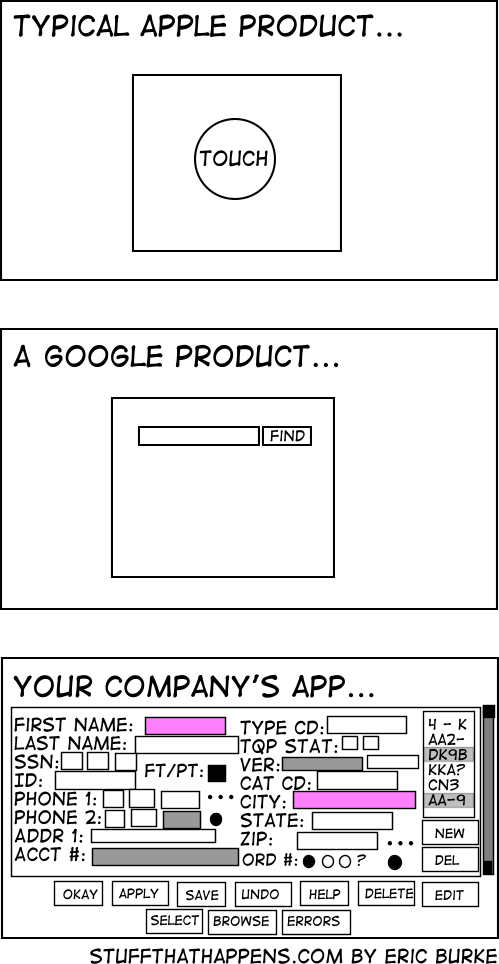
\includegraphics[scale=0.7]{Bild/Usability_Comic.jpg}
		\caption{Apple, Google, You by Eric Barcks}
	\end{figure}
	Nach dem die Notwendigkeit geklärt ist, sollte noch in Erfahrung gebracht was Entwicklern das Lernen erleichtert und welche Medien, wie eingesetzt werden können. 
	Interaktivität und flexible Nutzbarkeit des Lernstoffes fördern die Bereitschaft von Schülern sich in  Eigeninitiative mit Lehrinhalten zu beschäftigen \cite[S.32 ff.]{beck2000eigenstandiges}. Was in jungen Jahren funktioniert, sollte im Laufe der Zeit nicht völlig versagen. Davon ausgehend ist das Web als Medium die erste Wahl sowohl für die formale wie auch informelle Vermittlung von Usability und Softwareergonomie Inhalten. 
	%Nach dem E-Learning Hype der vergangenen Jahre wird nun klarer, dass Technik allein nicht gleich einen pädagogischen Mehrwert schafft. Die Kombination aus didaktischer Aufbereitung und interaktiver Medien versprechen mehr Erfolg. 
	
	Im folgenden wird davon ausgegangen, dass Interessierte sich für die Auseinandersetzung mit der Thematik Usability die Basiszertifizierung \ac{CPUX}-F des \ac{UXQB} auswählen um als "`Usability Professional"' zertifiziert zu werden. Hierfür gibt es zahlreiche Anbieter, die im folgenden auch Erwähnung finden, solange diese neben Präsenzseminaren auch E-learning Anwendungen und Plattformen bieten. 
	Die grundlegenden Konzepte, Begriffe und Definitionen werden vom \ac{UXQB} als PDF-Dokument veröffentlicht\cite{cpux-f}. Um das Selbststudium für die Basiszertifizierung zu erleichtern, soll im Rahmen des KOMET Projektes an der \ac{HTW Berlin} %Hochschule für Technik und Wirtschaft Berlin
	in Kooperation mit der artop GmbH - Institut an der Humboldt-Universität zu Berlin eine webbasierte Anwendung entwickelt werden\cite{KOMET}. 
		
		
	\section{Zielsetzung}
	Die nachfolgende Arbeit beschreibt die Konzeption für die bereits als Prototyp existierende Anwendung mit Methoden der Lernpsychologie, den gängigen E-learning Anwendungen und der "Gamification" von Lerninhalten. Unter der Fragestellung wie können die Lehrinhalte (Begriffe und Definitionen) des \ac{UXQB} Glossars am einfachsten vermittelt werden wird ein prototypisches Beispiel entwickelt welches eine alternative Aufbereitung des Glossars zum bestehenden Quiz bietet. "Lernen und Spielen sind keine Gegensätze" \cite{dewey1995erfahrung}
	ist der Leitspruch dem mit ausgewählten Aufbereitungsmethoden nachgegangen werden soll. Der Lernerfolg soll hierbei durch die Förderung der intrinsischen Motivation erzielt werden. 
	Primär soll in der nachfolgenden Arbeit das bereits als Prototyp entwickelte "`Usability-Quiz"' nach E-learning Methoden und Usability Richtlinien konzeptuell erfasst werden. Sekundär wird die weiter Entwicklung des Prototypen dokumentiert. Zum einen durch Zuordnung von Bildern zu den Begriffen zum anderen durch Kategorisierung der Begriffe um den Schwierigkeitsgrad zu steigern. Die didaktische Aufbereitung der Lehrinhalte sowie die Stärkung von Lernanreizen stehen im Mittelpunkt. Um einen Ausblick zu geben werden bestehende E-learning Angebote und Lernumgebungen erwähnt und zugeordnet. 
	%Primäres Ziel ist die zur Basis Zertifizierung bereit gestellten Begriffe und Definitionen so aufzubereiten, dass Interessierten der Stoff einfach zugänglich gemacht ein Lernanreiz geschaffen wird. Einen Lernerfolg erzielen, abhängig von der Definition eines Lernerfolges. Blickbewegungsanalysen
	%Wiedergeben können der Begriffe und Definitionen oder diese im Context von Usabilitytests anwenden können?
	
	%Kategorisierung der Usabilitybegriffe, streichen der Synonyme bzw. neue Fragestellung mit englischen Begriff bzw. den Synonymen, z.B. Unter welchem Begriff ist ... noch bekannt. 
	\section{Aufbau der Arbeit}
	Am Beispiel ausgewählter \ac{BUIS} wird unter Kapitel 2 die Umsetzung des Usability Glossar des \ac{UXQB} aufgezeigt und die Schulungsangebote erwähnt. Was unter Usability verstanden wird und welches Wissen darüber vermittelt werden soll ist unter Kapitel 3 zu finden. 
	% zum anderen der Einsatz von E-learning und Tutorials aufgezeigt.  
	
	In Kapitel 4 werden die gängigen Lerntheorien und Ihre Umsetzung beim lernen mit E-learning Anwendungen beschrieben. Hauptaugenmerk bei der Entwicklung der E-learning Anwendung soll die spielerische Umsetzung (Gamification) und Didaktische Aufbereitung von Lehrinhalten sein. 
	Mit diesem Grundlagenwissen sowie den technischen Details wird unter Punkt 5 das Konzept beschrieben und die Umsetzung dokumentiert. 
	Zum Abschluss wird noch einmal zusammengefasst was umgesetzt wurde und welche Potentiale noch in der Entwicklung des Usability Quiz stecken. 
	
	\chapter{Theoretische Grundlagen BUIS}
In diesem Kapitel werden die grundlegenden theoretischen Hintergründe zum Verständnis der Arbeit erläutert.
	\section{Definition}
	„Ein \ac{BUIS} %Betriebliches Umweltinformationssystem (BUIS)
	ist eine Softwareanwendung, die für die Erfassung, Dokumentation und Bewertung betrieblicher Umweltwirkungen sowie  zur Generierung, Planung und Steuerung von Umweltschutzmaßnahmen genutzt wird und damit das betriebliche Umweltschutzmanagement in seinen Aufgaben unterstützt.“ \cite{wohlgemuth2008konzepte}
	"Ein BUIS erfasst, verarbeitet und gibt umweltrelevante Daten aus und dient damit der Quantifizierung und Bewertung der Einflüsse unternehmerischen Handelns auf die natürliche Umwelt."'\cite{Wiki_BUIS} `
	Die verfügbaren Definitionen des Begriffs \ac{BUIS} lassen sich grundsätzlich durch einen
	organisatorischen und einen informationstechnisch geprägten Zugang zu dem Thema erklären. Die erste Definition schließt den organisatorischen und technischen Teil Umweltrelevanter Informationen mit ein. Im Unternehmenskontext lassen sich \ac{BUIS} den betrieblichen Informationssystemen den sog. \ac{ERP} Systemen zuordnen. 
	Ein \ac{BUIS} kann demnach für die interne Dokumentation, für den Austausch mit Behörden oder der Öffentlichkeit angelegt sein, es kann Aufgaben bei der Planung und Kontrolle von Maßnahmen innerhalb	des Umweltmanagements übernehmen oder operative Funktionen z.B. der Rechtssicherheit erfüllen. In der EMAS - Verordnung werden \ac{BUIS} als informationstechnisches Werkzeug für eine effiziente Umsetzung dieser Verordnung gesehen\cite[S. 109ff]{rautenstrauch1999betriebliche}.  
	 In älteren Nutzungskontexten wurden Anwendungen wie die manuell erstellte Umweltbilanz über Tabellenkalkulationen bereits als \ac{BUIS} bezeichnet. Aktuell und nach der Wikipedia Definition ist eine spezifische Software mit konkreten Aufgaben als \ac{BUIS} betitelt. Um der Komplexität der genannten Aufgaben gerecht zu werden sind die meisten Anwendungen selbst vielschichtig und komplex.
	
	\section{Kategorisierung}
	 \ac{BUIS} verfolgen einen ganzheitlichen Ansatz werden dennoch meist punktuell und für die konkreten Bedürfnisse in \ac{KMU} entwickelt. Dies führt dazu, dass nicht der Nutzer zentrierte Ansatz bei der Entwicklung verfolgt wird, sonder meist der Nutzen zentrierte. Die meisten \ac{BUIS} basieren auf dem Tabellenverarbeitungsprogramm Microsoft Excel und folgen den gleichen Handlungsanleitungen zur Erfüllung der Aufgaben. 
	Eine Übersicht nach welchen Merkmalen \ac{BUIS} klassifiziert werden können und welchen Funktionsumfang Sie abdecken gibt der Morphologische Kasten.
	
	\begin{figure}[h!]
		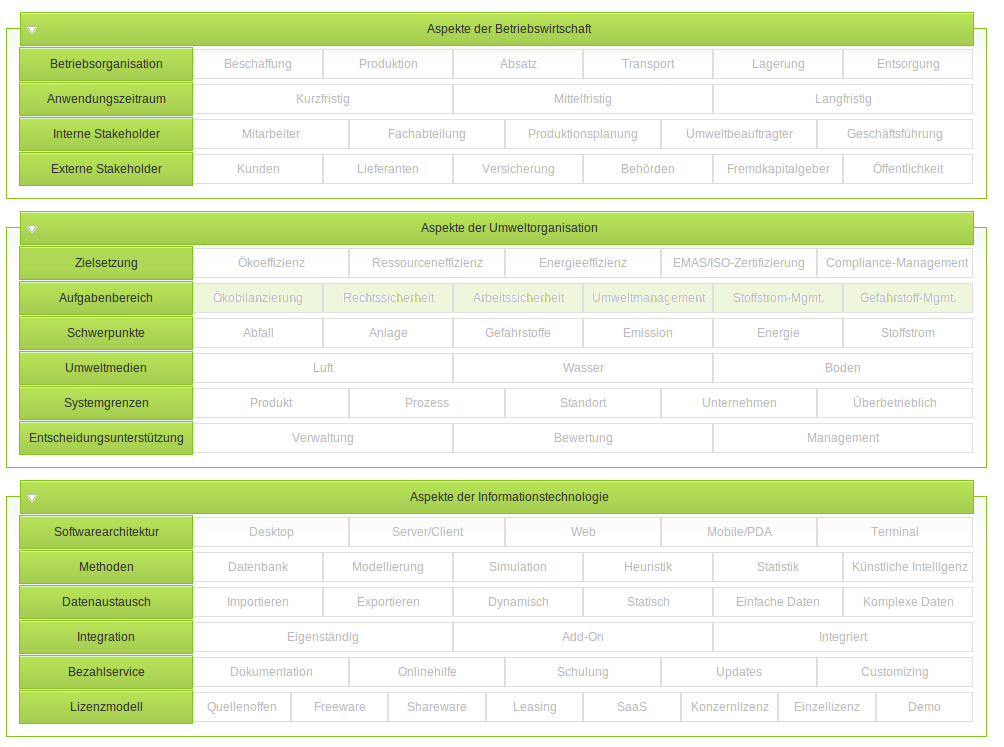
\includegraphics[width=\textwidth]{Bild/Morphologischer_Kasten_BUIS_Talus.png}
		\caption{Morphologischer Kasten}
		\quelle{}
	\end{figure}
	
	Ausgehend von den markierten Aufgabenbereichen sollen 3 \ac{BUIS} als Repräsentanten für Ihren Nutzungskontext näher beleuchtet werden. Das Augenmerk liegt dabei auf der Erfüllung der Empfehlungen der DIN ISO EN 9124 (Teil 210 Ergomomics of human-centred design processes for interactive systems/ Ergonomie der Mensch-System-Interaktion) \cite{ISO9241}. Die Begriffsklärung für Usability und die in der ISO Norm genutze Terminologie ist unter Kapitel 3 erklärt und zugeordnet. Die Normenreihe ISO 9241 umfasst über 400 Empfehlungen für fast alle Bereiche der Softwaregestaltung. Somit sollte klar sein, dass nur einige Designempfehlungen herangezogen werden siehe Abbildung.
	\begin{figure}[ht]
			\centering
			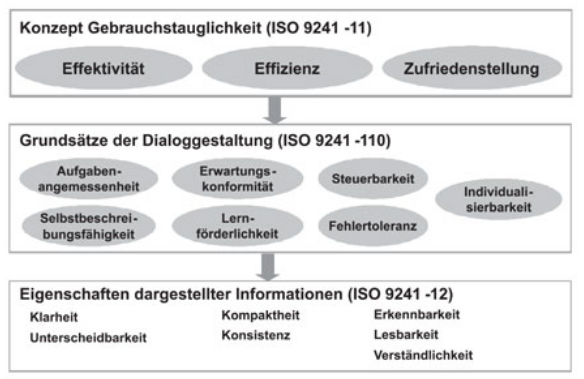
\includegraphics[width=\textwidth]{Bild/Normenteile ISO 9241-11, 9241-110, 9241-12 Dialoggestaltung Software-Ergonomie.png}
			\caption[ISO 9124 Verhältisse der Normenreihe]{ISO 9124 Verhältisse der Normenreihe\cite{ISO9241Bild}} 
		\end{figure}

%	 ISO 9126 Qualitätskriterien für Software\cite[S.463ff]{balzert2009lehrbuch} siehe Abbildung 2.2 und der Umsetzung der
%	\begin{figure}[ht]
%		\centering
%		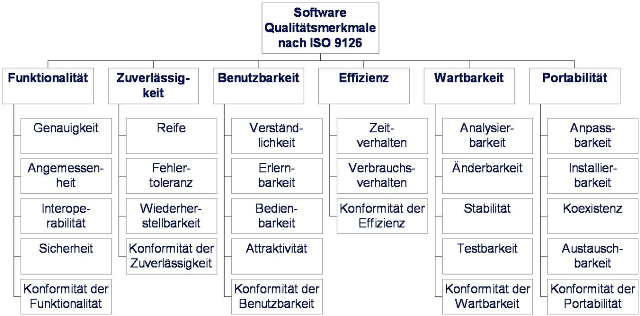
\includegraphics[width=\textwidth]{Bild/ISO 9126 WI Balzert S463ff.png}
%		\caption[ISO 9126 Qualitätsmerkmale von Software]{ISO 9126 Qualitätsmerkmale von Software laut Balzert 2008, S. 463ff\cite{balzert2009lehrbuch}} 
%	\end{figure} 
	
	Weiterhin finden die Schulungs- und Weiterbildungsangebote ausgewählter \ac{BUIS} Erwähnung, um potenzielle Einsatzmöglichkeiten von E-Learning Angeboten aufzuzeigen.  
	%Teil 210: Prozess zur Gestaltung gebrauchstauglicher interaktiver Systeme (Ersatz für die EN ISO 13407)
	
	\section{Nutzungskontext und Softwareergonomie: Konformität ausgewählter \ac{BUIS}}
	Aus einer Vielzahl von Anwendungen und Software wurden die folgenden nach der Verfügbarkeit von Zugängen und Demoversionen ausgewählt. Die folgenden Screenshots und dazugehörigen Anmerkungen dienen als Beispiel für die Unterstreichung des Thema Usability und E-learning im Kontext betrieblicher Umweltinformationssysteme und sind keine Ergebnisse einer Wissenschaftlichen Erhebung. 
	%die Browser basierte Software der Ecointense GmbH der Repräsentant für Rechtssicherheit Software(Legal Comliance). \\
	\begin{enumerate}
	\item Umberto der ifu Hambug GmbH dient als Beispiel für ein Umweltmanagementsystem zur Prozessoptimierung.\\
	\item Die webbasierte SimaPro Software der GreenDelta GmbH ist Vertreter für Ökobilanzierungssoftware. \\
	\item eSankey, die Visualisierungssoftware für Stoff- und Energieströme ebenfall aus dem Hause ifu Hamburg GmbH dient als Repräsentant für ein Stoffstrommanagement. 
	\item EcoWebDesk als Umweltmanagement Software für Rechtssicherheit mit dem Modul - Legal Compliance
	\end{enumerate}

Die Herangehensweise ist folgende: Als Mitarbeiter eines Unternehmens in dem das ausgewählte \ac{BUIS} neu eingeführt wurde, sollen die Alltagsgeschäfte damit durch geführt werden. Das bedeutet im Fall von SimaPro, erstelle ich eine Ökobilanz für ein Produkt unseres Unternehmens. Im Fall von e!Sankey skizziere ich Diagramme zu den Prozessen im Unternehmen. Mit Umberto wird der Produktionsprozess eines Produktes mit all seinen Material- und Energieströmen modelliert um Optimierungspotentiale zu entdecken. EcoWebDesk möchte keine vergleiche und wird daher nur mit den Schulungsangeboten aufgeführt.    
Folgende Fragen sollen beantwortet werden:
\begin{itemize}
\item Wie sieht die Startseite aus?
\item Wo befindet sich die Navigation und ist mir diese schon bekannt?
\item Wo und wie ist Hilfe zu finden?
\item Sind Inhalte klar und deutlich benannt und gestaltet?
\item Gibt es Handlungsanweisungen?
\item Wie wird auf Fehlverhalten aufmerksam gemacht?
\item Ist der Arbeitsbereich personalisierbar?
\end{itemize}
	
\subsection{Umberto NXT der ifu Hamburg GmbH - Umweltmanagemetsystem} 

	Umberto ist eine besonders komplexe Stoffstrommanagement Software, die eine Bandbreite an Anwendungsmöglichkeiten bietet. Von der Ökobilanzierung zur Simulation von Prozessen und Ihrer Visualisierung deckt es alle Anforderungen an ein Stoffstrommanagement Tool. %, vorausgesetzt man weißes zu nutzen.
	Umberto findet Anwendung in der Strategischen Planung von \ac{KMU} unter der Fragestellung "`Mit welchem Maßnahmen-Mix erreichen wir am besten unsere Innovations-, Umwelt- und Kostenziele?"'
%\item Wie sieht die Startseite aus?
%\item Wo befindet sich die Navigation und ist mir diese schon bekannt?

%
%\item Wo und wie ist Hilfe zu finden?
%\item Sind Inhalte klar und deutlich benannt und gestaltet?
%\item Gibt es Handlungsanweisungen?
%\item Wie wird auf Fehlverhalten aufmerksam gemacht?
%\item Ist der Arbeitsbereich personalisierbar?		
	\begin{figure}
	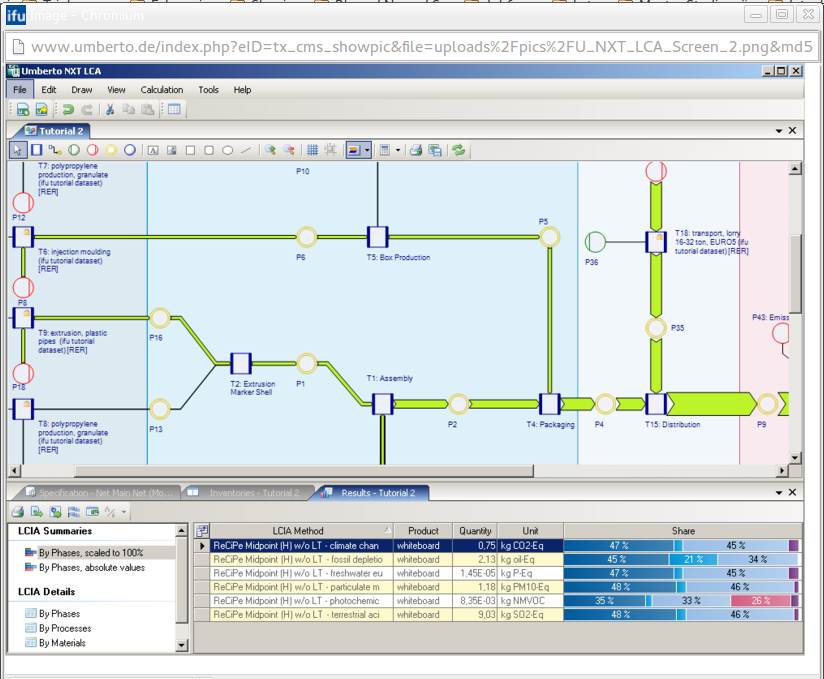
\includegraphics[width=\textwidth]{Bild/Umberto_NXT_LCA.png}
%		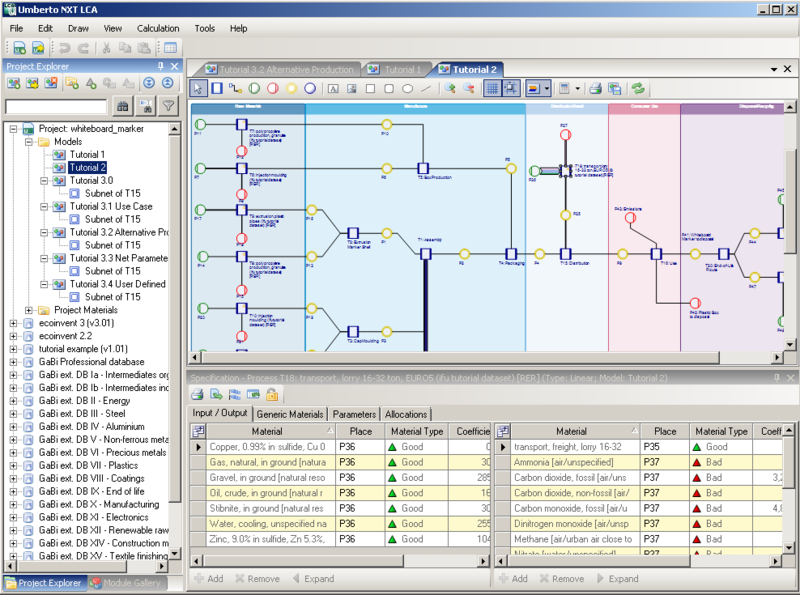
\includegraphics[width=\textwidth]{Bild/Umberto NXT LCA.png}
		\caption{Umberto LCA Beispielbild} 
	\end{figure}
	
	Im der Abbildung Umberto LCA sind Beispielhaft einige Positionen markiert, die den Usability Richtlinen nicht gerecht werden. 
	Trotz der Komplexität des Programmes, gäbe es an den Markierten punkten Verbesserungspotentiale zur Benutzbarkeit der Software. 
	
\subsection{Sima Pro - Ökocontroling}
\subsubsection{Ökobilanzierung}
Der deutsche Begriff Ökobilanzierung ist besser bekannt als \ac{LCA}zu deutsch eine Lebenszyklusanalyse und wird in dieser Arbeit verwendet\cite{klopffer2009okobilanz}.
Die Norm DIN EN ISO 14040 "Umweltmanagement - Produkt-Ökobilanz - Prinzipien und allgemeine Anforderungen" sowie die darauf aufbauenden DIN EN ISO 14041, 14042 und 14043 geben die Schritte für eine Ökobilanz vor, um z. B. den Lebensweg eines Produktes "von der Wiege bis zur Bahre" analysieren und bewerten zu können. Die Norm kann in allen Branchen sowohl für Dienstleistungen als auch für Produkte angewendet werden.
\begin{figure}
\centering
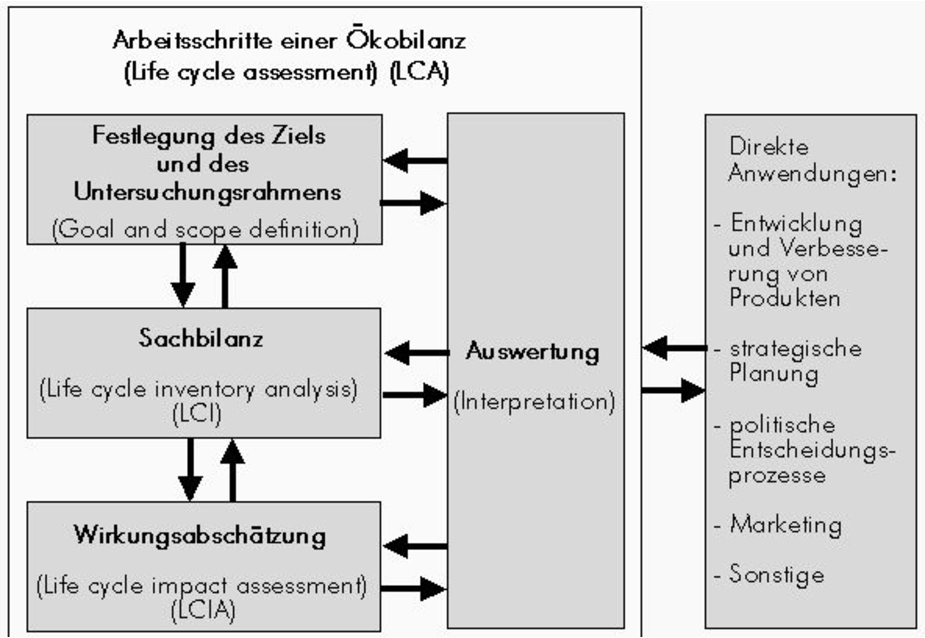
\includegraphics[width=\textwidth]{Bild/ISO 14040 Oekobilanz1.pdf}
\caption{Arbeitsschritte einer Ökobilanz nach ISO 14040\cite{klopffer2009okobilanz}}
\end{figure}

\subsubsection{SimaPro Compact}
SimaPro ist eine weltweit vertriebene Desktop Software für \ac{LCA} die Ihre Daten aus zahlreichen mitgelieferten Datenbanken bezieht. Von ELCD über LCA Food und nationalen Input/Output-Datenbanken bis zu ecoinventder Ecoinvet Datenbank sind die Lizensen beim Kauf von SimaPro inbegriffen\cite{SimaPro_Homepage}. Dies ist ein Vorteil im Vergleich zu OpenSource alternativen, bei denen die Datenbanken nicht inbegriffen sind. 
Nutzungskontext der SimaPro Compact Software ist, dass ein Mitarbeiter eines Unternehmens ein \ac{LCA} für ein bestehendes Produkt berechnen möchte. Die gewählten Mengen, Materialien sowie das Produkt sind fiktiv und stellen keine Grundlage für eine Berechnung dar.Ziel für unser Beispiel, wir möchten die CO2 Bilanz der Kaffeemaschine A mit der Kaffeemaschine B vergleichen. Das Szenario ist als Tutorial bereits in der Demoversion integriert.
%SimaPro provides you with a professional tool to collect, analyze and monitor the sustainability performance of products and services.
%\item Wie sieht die Startseite aus?
%\item Wo befindet sich die Navigation und ist mir diese schon bekannt?
%\item Sind Inhalte klar und deutlich benannt und gestaltet?
\begin{figure}{h}
\centering
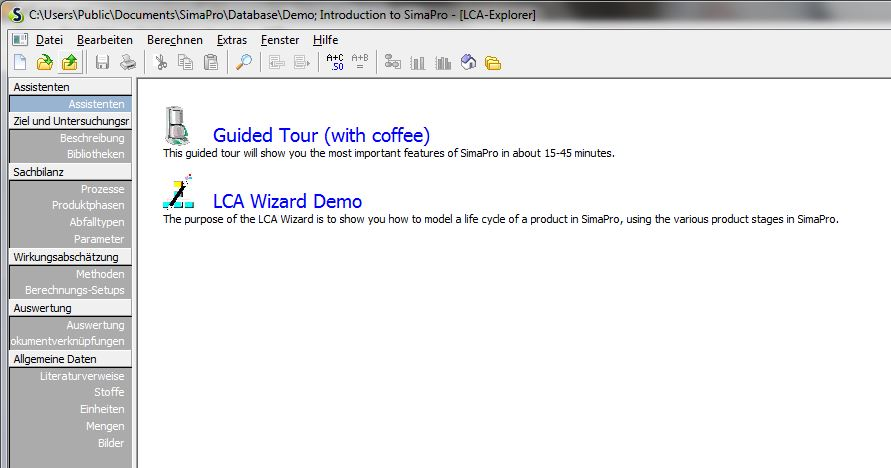
\includegraphics[width=\textwidth]{Bild/Sima Pro Start.JPG}
\caption{SimaPro Start Display der Demoversion Compact}
\end{figure}
Hilfe ist der Konverntionentsprechend in der oberen Menüleiste zu finden. Die Hilfeoptionen fallen besonders umfangreich aus durch verschiedene Handbücher auch zu den integrierten Datenbanken und des E-Mail Helpdesk.   
%\item Wo und wie ist Hilfe zu finden?
\begin{figure}{h}
\centering
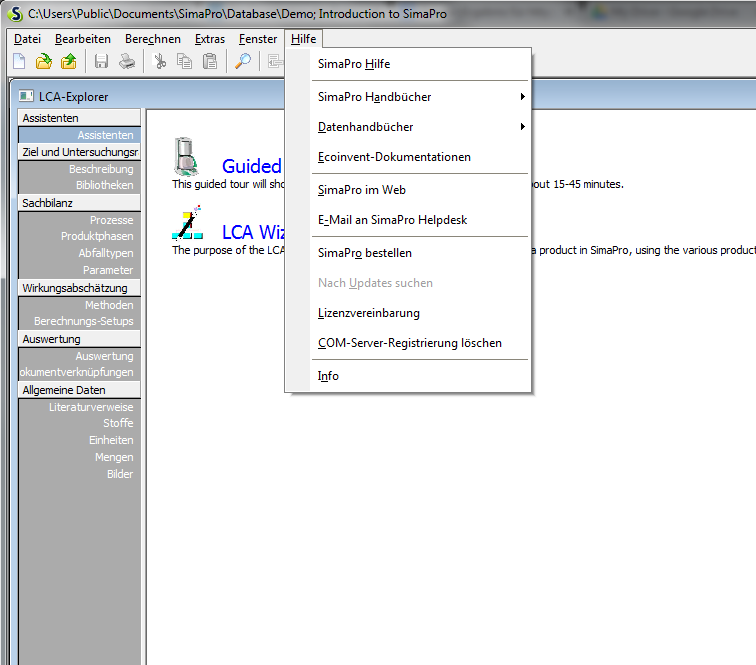
\includegraphics[width=\textwidth]{Bild/SimaPro Hilfe.png}
\caption{SimaPro Hilfe}
\end{figure}
%\item Gibt es Handlungsanweisungen?
%\item Wie wird auf Fehlverhalten aufmerksam gemacht?
%\item Ist der Arbeitsbereich personalisierbar?
Die Abbildung zeigt den Wizard, wie er den Nutzer Schritt für Schritt durch den Entwicklungsprozess leitet. Der Dialog ist vom Nutzer frei zu starten, fortzusetzen, Einzelschritte zu wiederholen und zu beenden. Ausgehend vom fertigen Produkt(siehe Markierung 3. in Abbildung 2.6) fragt der Wizard ob Material oder ein Prozess hinzugefügt werden soll.  
Die Markierung 1. in Abbildung 2. kennzeichnet die Navigation, welche den Erwartungen der meisten Windows Nutzer entspricht und den Konventionen von Desktop-basierter Software. 
%sowie den Kenntnissen eines Mitarbeiters im Bereich des Umweltmanagement. 
Die Legende unter 2. in Abbildung 2. zeigt mehr als nötig, ist weder skalierbar noch veränderbar was Farbgebung angeht. 
\begin{figure}[h]
\centering
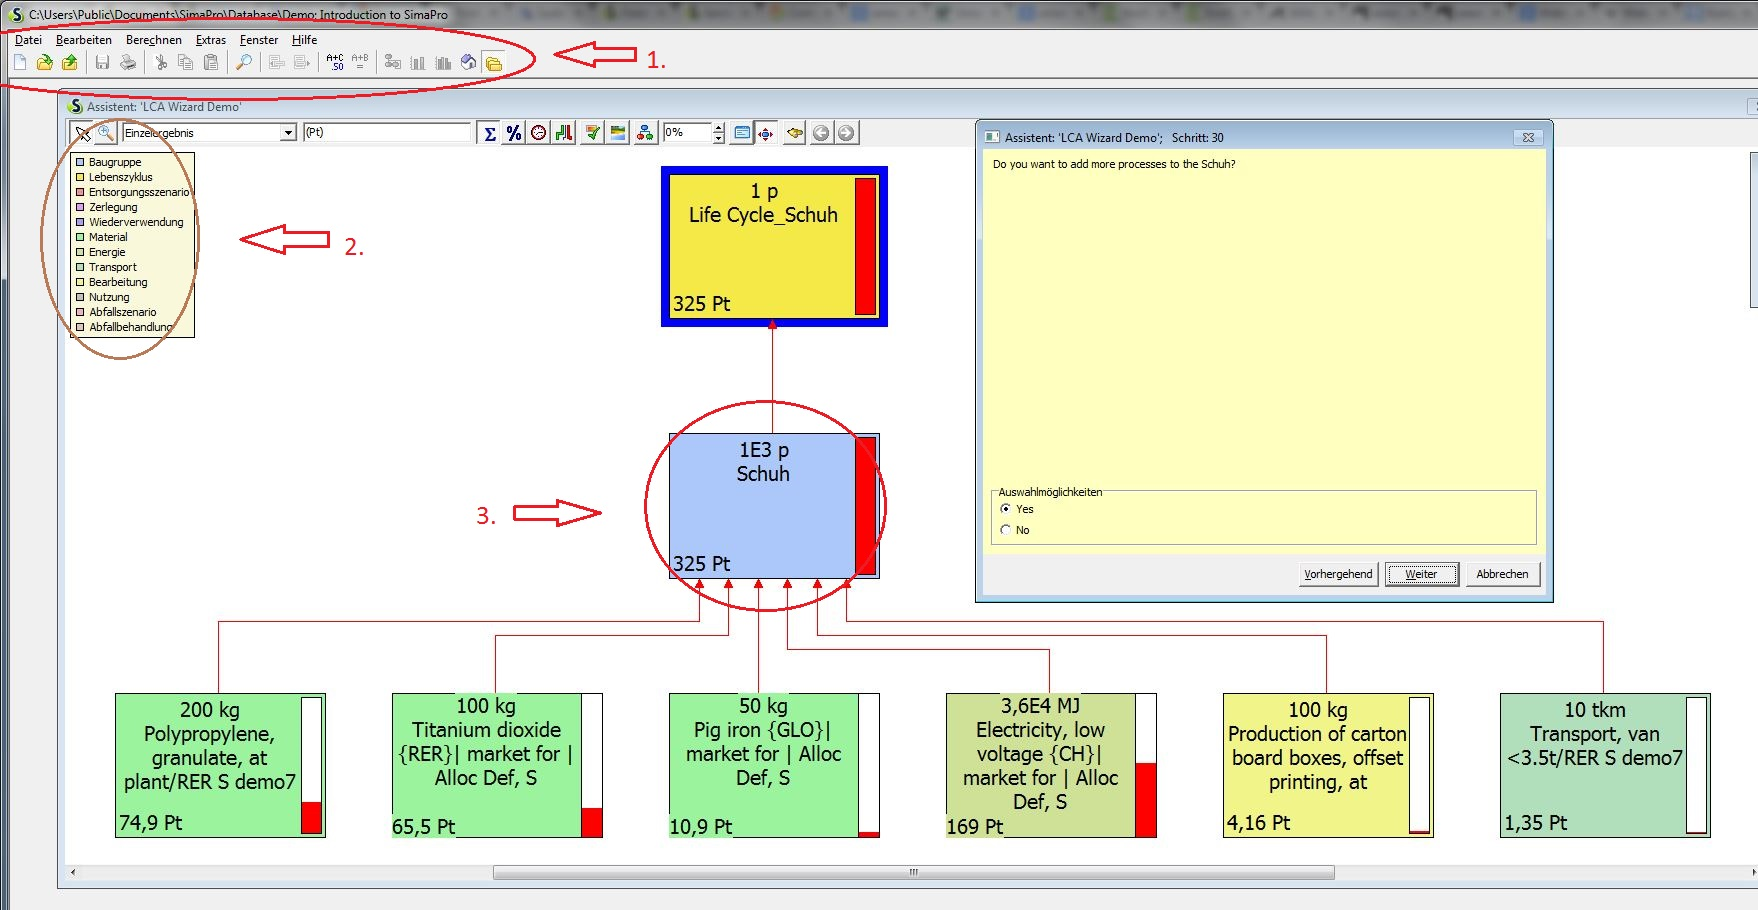
\includegraphics[width=\textwidth]{Bild/SimaPro LCA Demo Material Process.JPG}
\caption{SimaPro LCA Wizard Demo}
\end{figure}
Die Datenbankinformationen berufen sich auf einige Annahmen die nicht herausgestellt werden. Dies verleitet zur Absolution des \ac{LCA} und der Prozesse, was nicht der Realität und den tatsächlich verfügbaren Daten entspricht. 
Die \ac{LCA} Prozesse werden lediglich nach dem Bottem-Up-Prinzip visualisiert, jedoch nach dem Top-Down Prinzip modelliert. Die Veränderung der Darstellung ist dem Nutzer nicht möglich.
Über den LCA Explorer lassen sich Prozesse, Produktphasen, Abfalltypen, Parameter, Methoden und Berechnungs-Setups hinzufügen, verändern und wieder entfernen. Diese Funktionen sind zwar erwartungskonform, gewähren jedoch kaum Fehlertoleranzen, da die Eintragung eines neuen Parameter nur erfolgt, wenn der Datensatz vollständig eingegeben wird. 

\begin{figure}
\centering
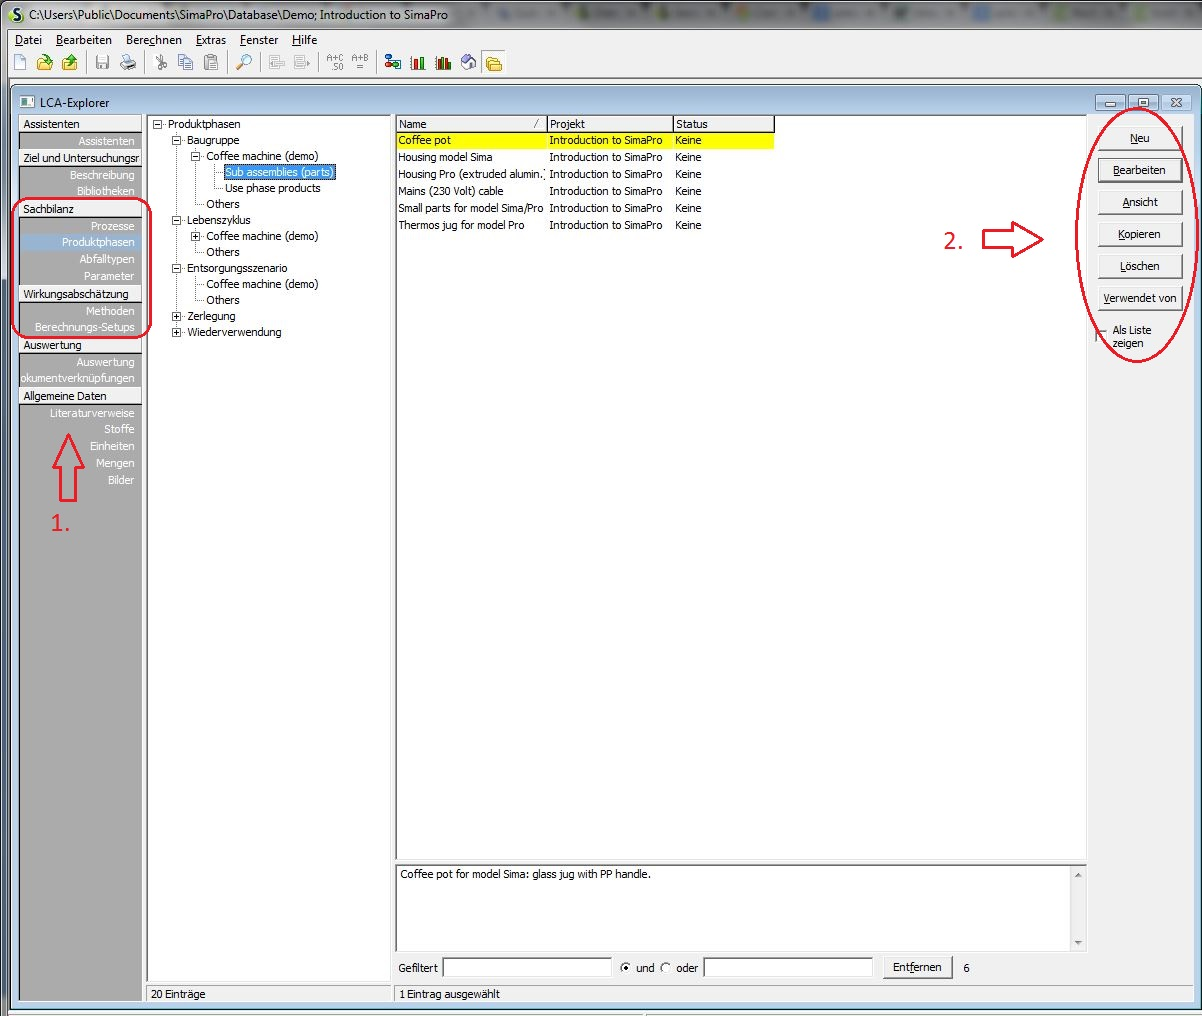
\includegraphics[width=\textwidth]{Bild/Sima Pro Coffee Prozesse.JPG}
\caption{SimaPro LCA Explorer}
\end{figure}
Im LCA-Explorer ist jedes Element anklickbar, wird jedoch nicht so gekennzeichnet. Der Kursor verändert sich nicht und bietet auch keine Informationen zum Untergrund beim drüberfahren. Dies sind kleine Hilfestellungen für die Steigerung der Usability von SimaPro.  

\subsubsection{Schulungen und E-Learningangebote}
Die Demoversion der SimaPro Software bietet zwei Einführungsfunktionen in die Nutzung des \ac{LCA}-Tool. Für eine Einführung in die wichtigsten Funktionen von SimaPro die "Guided Tour(with coffee)" und der LCA Wizard demonstriert die Modellierung eines \ac{LCA} für ein spezifisches Produkt. siehe Abbildung 

Neben diesen interaktiven Methoden gibt es natürlich noch das Handbuch und die Dokumentation als PDF. 
Präsenzschulungen werden sowohl inhouse, online sowie wie auch in den Räumen der GreenDelta GmbH für Gruppen wie Einzelpersonen angeboten. Die Schulungen sind Kompaktkurse, die über 1,5 Tage gehen und ohne Zertifikat abschließen. Die Onlineschulung ist ein Webinar (Web Seminar), welches derselben didaktischen Aufbereitung des Präsenzseminars entspricht und lediglich die Übungsphasen und Selbstversuche der Teilnehmer außen vor lässt.  
%\begin{figure}{h!}
%\centering
%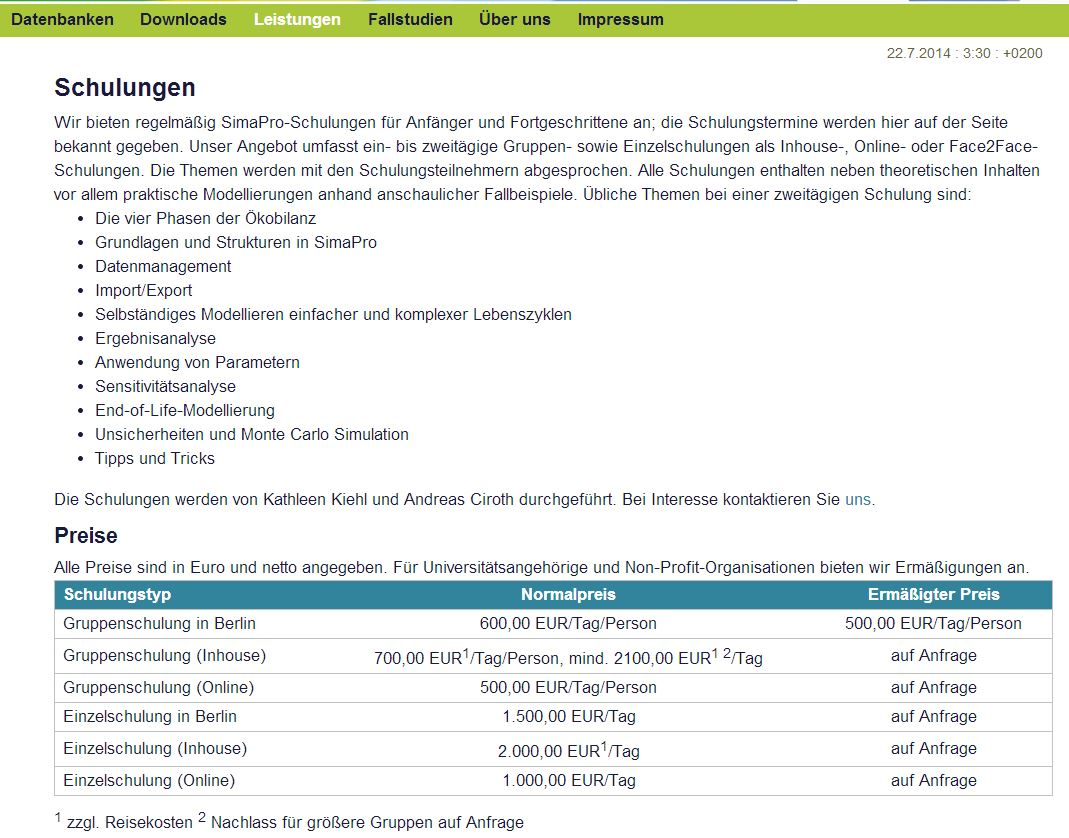
\includegraphics{Bild/Sima Pro Schulungsangebot.JPG}
%\caption{Schulungsangebot von SimaPro}{Schulungsangebot von SimaPro laut \cite[Website vom 13.07.2014]{SimaPro_Homepage}}
%\end{figure}

\subsection{e!Sankey (ifu) - Stoffstrommanagement Visualisierung}
	\subsubsection{Stoffstrommanagement - Visualisierung}
Stoffstrommanagement wird meist verstanden als eine Analyse- und Optimierungsmethode von Material und Energieströmen im Produktionsprozess\cite[S. 167]{wohlgemuth2005komponentenbasierte}. Eine frühe Definition findet sich in einem Bericht der Enquete-Kommission des Deutschen Bundestages:
"Unter dem Management von Stoffströmen der beteiligten Akteure wird das zielorientierte, verantwortliche, ganzheitliche und effiziente Beeinflussen
von Stoffsystemen verstanden, wobei die Zielvorgaben aus dem ökologischen und dem ökonomischen Bereich kommen, unter Berücksichtigung von sozialen Aspekten. Die Ziele werden auf betrieblicher Ebene, in der Kette der an einem Stoffstrom beteiligten Akteure oder auf der staatlichen Ebene entwickelt.\cite[S. 259]{raey}

Stofftromanalysen können nach dem betrachteten Objekt oder nach gewählten Systemgrenzen unterschieden werden kann. Ein Produktorientiertes Stoffstrommanagement ist auch bekannt als \ac{LCA} und entspricht einer Ausprägung des Stoffstrommanagement. Die Stoff- und Ernergiestromanalyse nach betrieblichen Prozess bezogenen Grenzen ist eine weitere Form. Wie in der Nachfolgenden Abbildung deutlich wird, lassen sich für die verschiedenen Etappen des Analyseprozesses verschiedene Werkzeuge (Softwaretool) nutzen. Wie z.B. e!Sankey für die Visualisierung.
\begin{figure}
\centering	
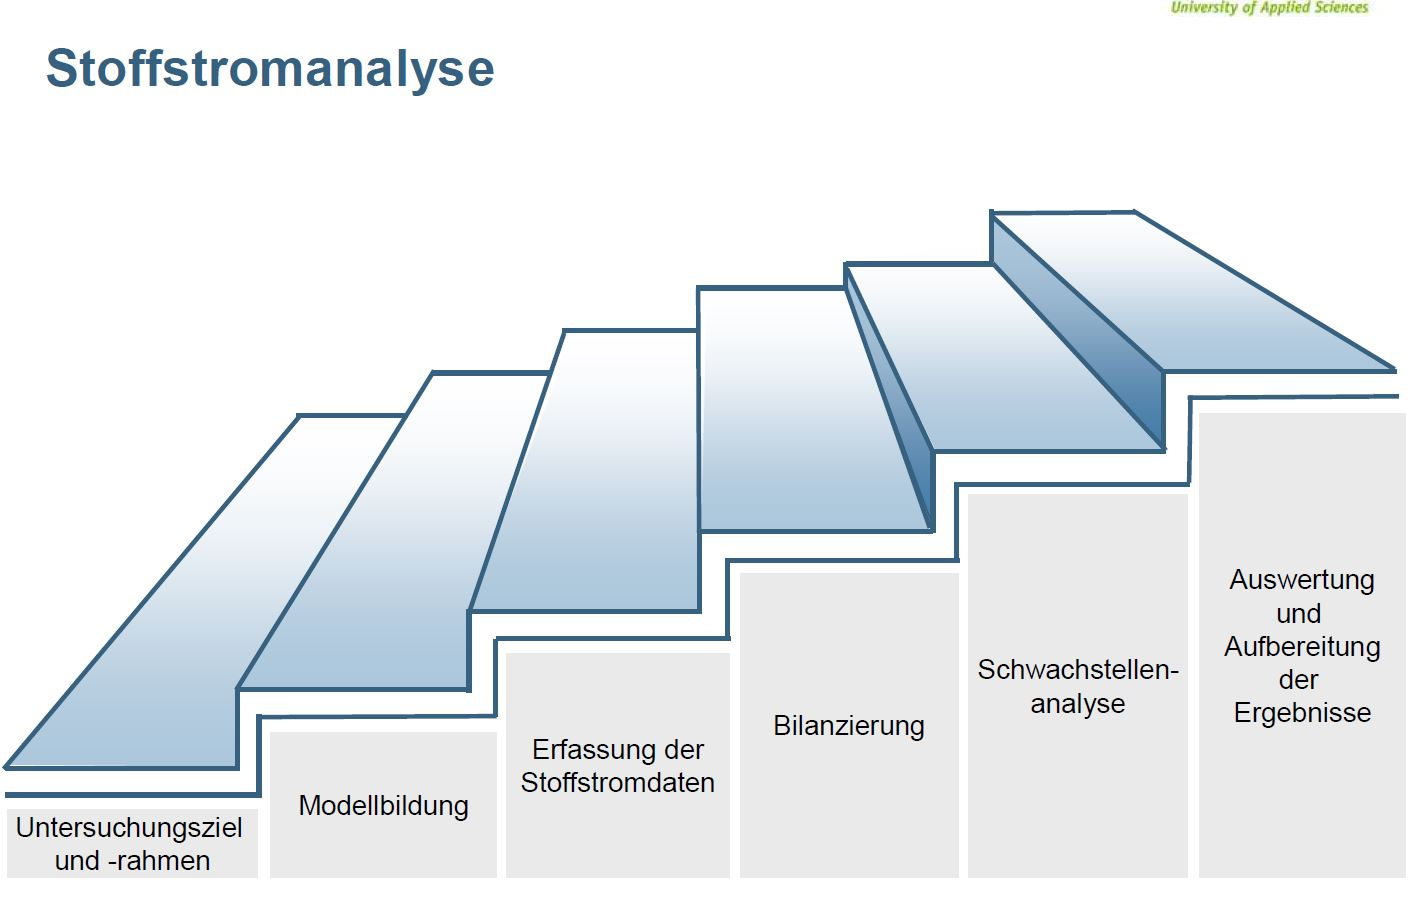
\includegraphics{Bild/Stoffstromanalyse.jpg}
\caption{Stoffstromanalyse Treppe}{Stoffstromanalyse Treppe laut Vorlesungsskript\cite{SAPSkript2011}}
\end{figure}

\subsubsection{e!Sankey}
e!Sankey als einfaches Stoffstrommanagement Tool, dient zur Visualisierung von Prozessen und Stoffströmen. Unter dem Motto "show the flow" lassen sich Flusskostenberechnungen farbenfroh und mit Logos oder Grafiken darstellen. 
%\item Wie sieht die Startseite aus?
%\item Wo befindet sich die Navigation und ist mir diese schon bekannt?
Die Begrüßung beim Programmstart, erfolgt nicht nur in der Demoversion mit einer Versionsinformation. Neben der Standartnavigation oben links, gibt es einen schnell zugriff auf die zuletzt bearbeiteten Projekte im linken Navigationsfenster. Für Neuanfänger finden sich in der Navigation Beispiele und Vorlagen die mit einem Doppelklich ausgewählt werden können.  
\begin{figure}{h}
\centering
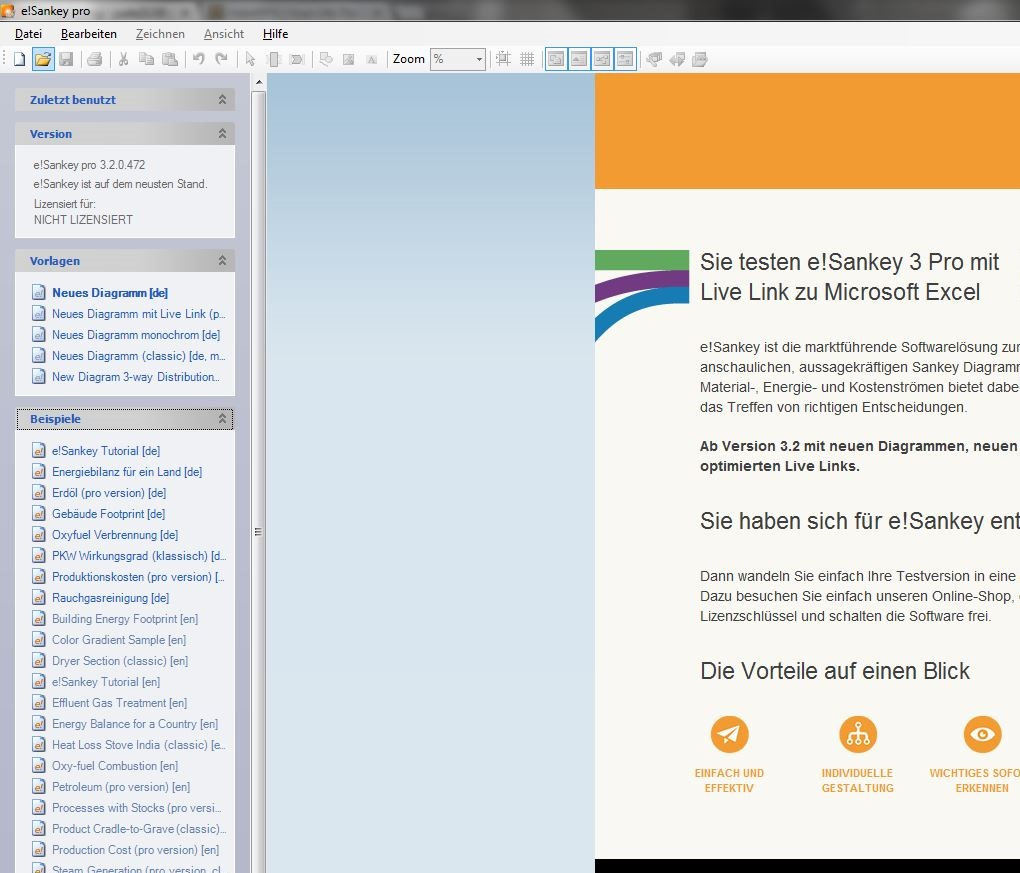
\includegraphics[width=\textwidth]{Bild/Esankey Start 2.JPG}
\caption{e!Sankey Startdisplay}{e!Sankey Startdisplay}
\end{figure}	
%\item Wo und wie ist Hilfe zu finden?
Unter dem Menüpunkt Hilfe ist wie zu erwarten diese zu finden. Ob im Handbuch, das Userforum im Web oder auf der Homepage von e!Sankey lässt sich Hilfe finden. 
\begin{figure}{h}
\centering
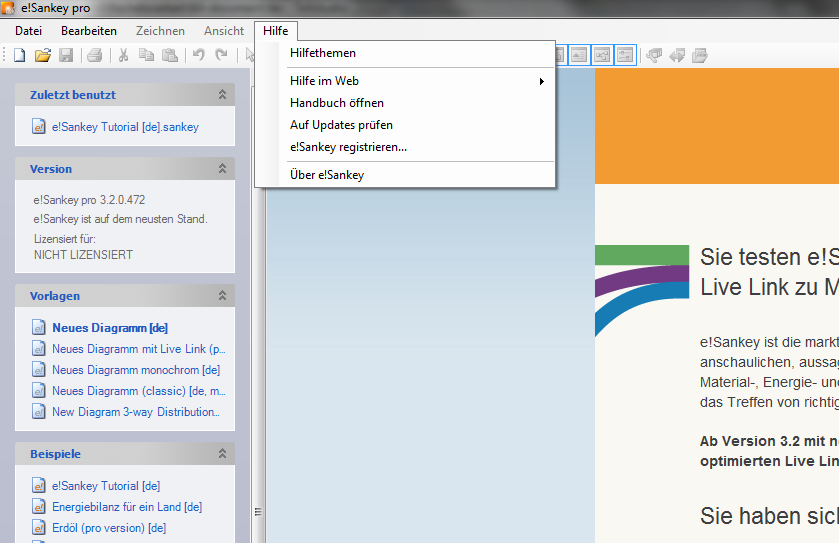
\includegraphics[width=\textwidth]{Bild/esankey Hilfe.png}
\caption{e!Sankey Hilfe}{e!Sankey Hilfe}
\end{figure}	
%\item Sind Inhalte klar und deutlich benannt und gestaltet?
%\item Gibt es Handlungsanweisungen?
%\item Wie wird auf Fehlverhalten aufmerksam gemacht?
%\item Ist der Arbeitsbereich personalisierbar?
Nach dem anklicken einer Vorlage gibt es verschiedene Anweisungen die man befolgen kann, zum Beispiel die Überschrift einfügen. Sowohl Informationsfenster wie auch Warnungen erscheinen als kleine Popup Fenster. Auf der linken Seite bleibt die Navigation erhalten und wird durch Optionen ersetzt. Die Optionen sind erweiterbar und das Arbeitsfeld mit kleinen Funktionen personalisierbar, z.B. der Hintergrundfarbe. Sollten Prozesse oder Pfeile integriert sein wie in der Abbildung 2. können diese mithilfe der Optionsleiste auf der rechten Seite skaliert werden. 
\begin{figure}{h}
\centering
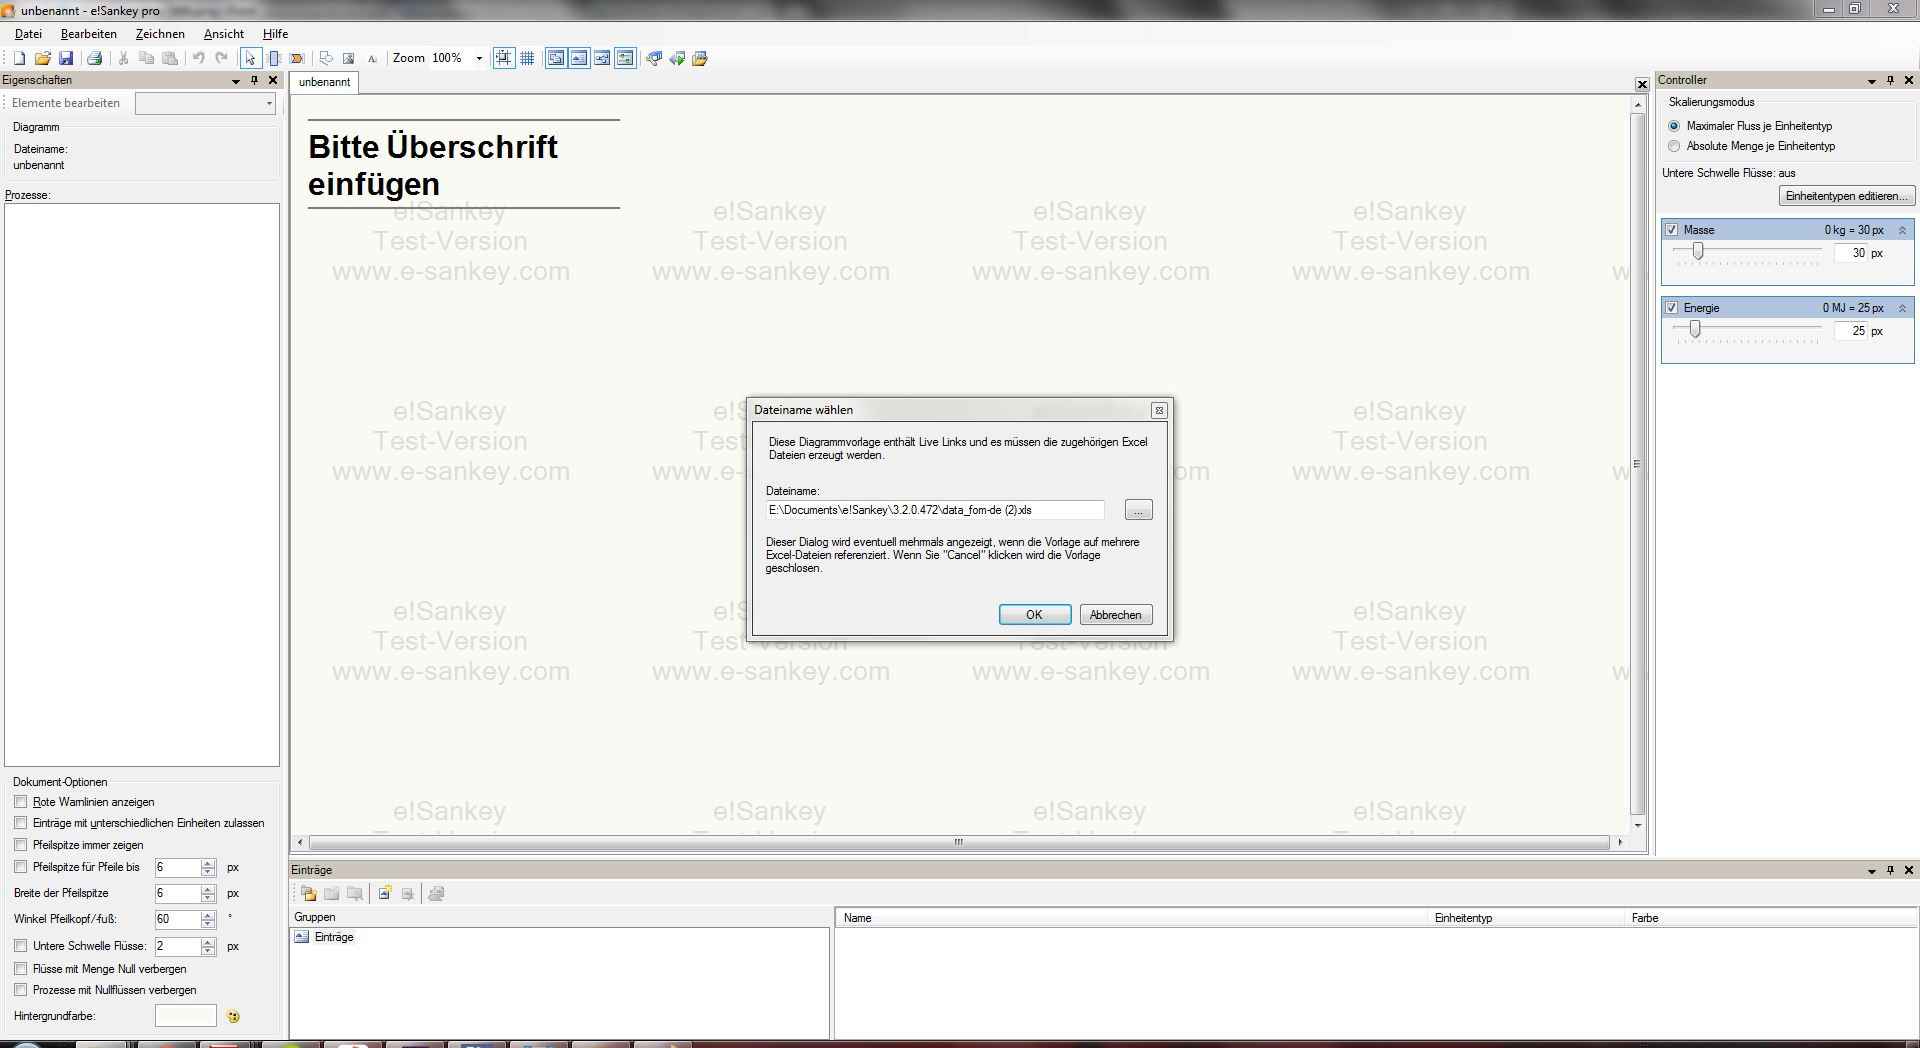
\includegraphics[width=\textwidth]{Bild/esankey Handlung und Infofenster.JPG}
\caption{e!Sankey Infofenster}{e!Sankey Infofenster}
\end{figure}	
Die Kurztasten in der oberen Leiste bieten die Möglichkeit den Arbeitsbereich zu Zoomen und eingeblendete Optionsfenster auszublenden. Für einen Nutzer mit Grundkenntnissen über Microsoft Office Anwendungen ist das modelieren eines Diagramms einfach. e!Sankey verhält sich Erwartungskonform und bietet eine konsistente Benutzerschnittstelle. 
\begin{figure}{h}
\centering
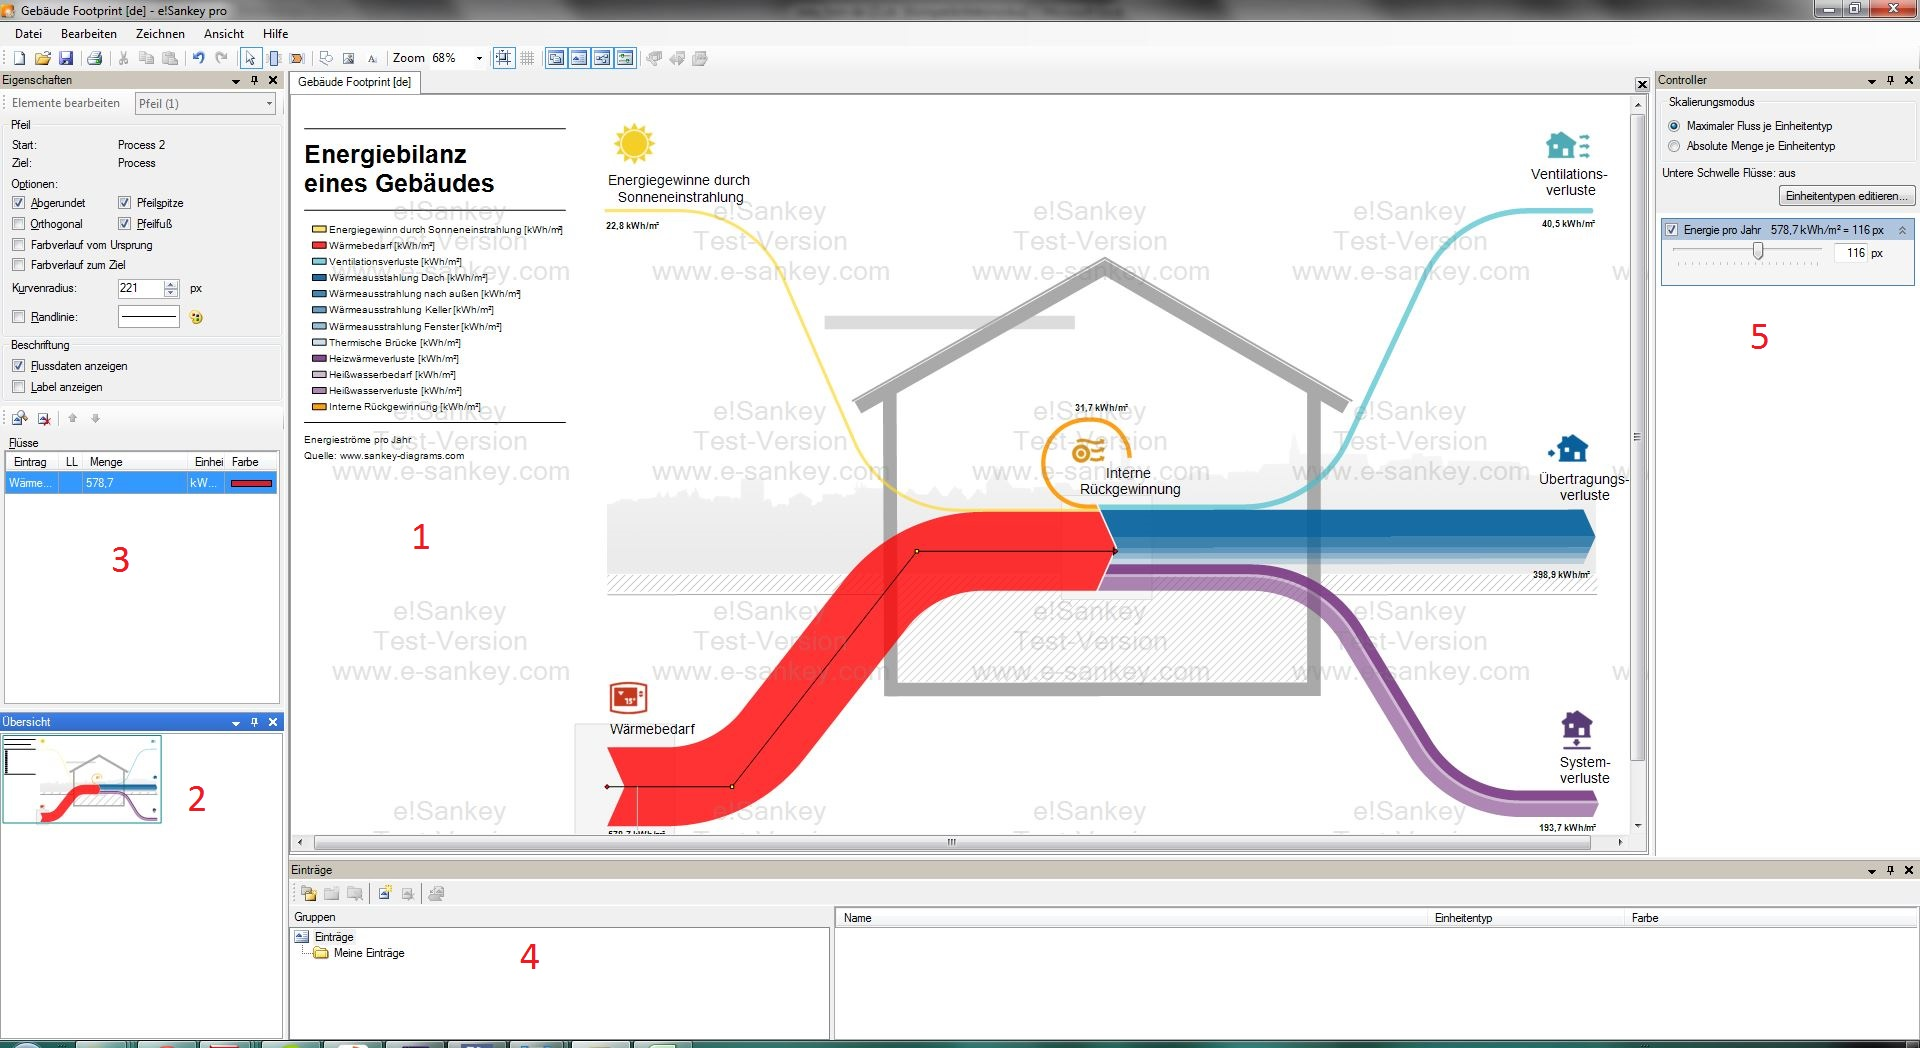
\includegraphics[width=\textwidth]{Bild/esankey Prozess Haus.JPG}
\caption{e!Sankey Prozess Energiebilanz}{e!Sankey Prozess Energiebilanz}
\end{figure}	
Dinge die sich von selbst erklären?
	1. Die Zeichenfläche (mehrere Diagramme können gleichzeitig geöffnet werden) 
	2. Übersicht: zeigt eine verkleinerte Ansicht des Sankey-Diagramms 
	3. Eigenschaften: ermöglicht die Bearbeitung der Eigenschaften von markierten
	Elementen 
	4. Einträge: Auflistung von Materialien, Energie und benutzerdefinierten Einträgen,
	die in den Pfeilen als Flüsse des Sankey-Diagramms verwendet werden 
	5. Controller: ermöglicht die Skalierung von Flüssen nach Basiseinheiten (kg, MJ) 


% und sich mit einem klick von aus einer Umberto Kalkulation erstellen lassen:
%\begin{figure}{h!}
%\centering
%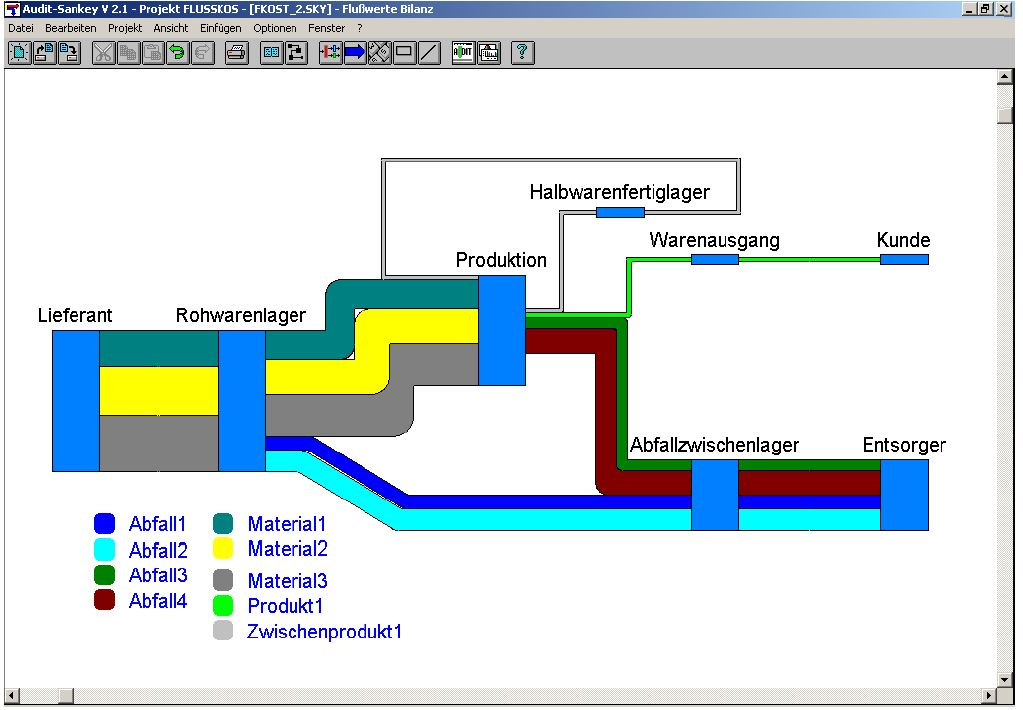
\includegraphics[width=\textwidth]{Bild/Audit-Sankey.JPG}
%\caption{Audit-Sankey}{Audit-Senkey Flussmengendarstellung \cite[S.40]{jurgens2001anforderungen}}
%\end{figure}	
%
%\begin{figure}
%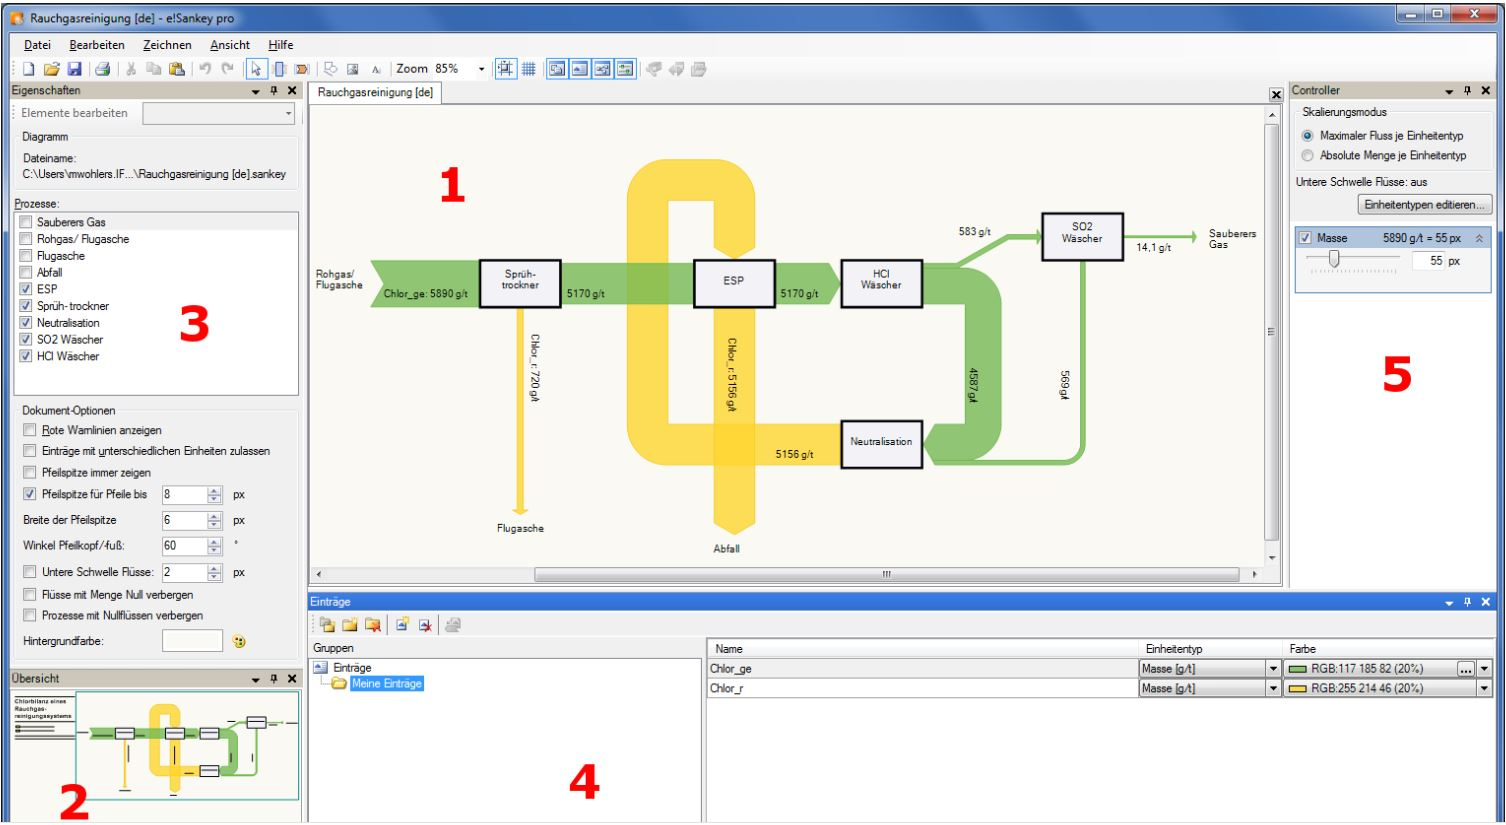
\includegraphics{Bild/Esankey Arbeitsbereiche Rauchgas.JPG}
%\caption{e!Sankey Arbeitsbereiche}{e!Sankey Arbeitsbereiche\cite{esankeyHandbuch032014}}
%\end{figure}
%Dinge die sich von selbst erklären?
%	1. Die Zeichenfläche (mehrere Diagramme können gleichzeitig geöffnet werden) 
%	2. Übersicht: zeigt eine verkleinerte Ansicht des Sankey-Diagramms 
%	3. Eigenschaften: ermöglicht die Bearbeitung der Eigenschaften von markierten
%	Elementen 
%	4. Einträge: Auflistung von Materialien, Energie und benutzerdefinierten Einträgen,
%	die in den Pfeilen als Flüsse des Sankey-Diagramms verwendet werden 
%	5. Controller: ermöglicht die Skalierung von Flüssen nach Basiseinheiten (kg, MJ) 
%	
%	Exklusiv bei e!Sankey pro: 'Live Link to Microsoft Excel', der automatisierte Import von Flusswerten aus Microsoft Excel Tabellenkalkulations-Dateien (erfordert Microsoft Excel 2002 oder höher)
%	Export des Sankey-Diagramms als Grafik (BMP, GIF, JPG, EMF, PNG)
%	Export als .sankey Datei (kann von anderen Tools z.B. Umberto gelesen werden)
%	Einstellung der Bildqualität beim Export (geringe Auflösung/hohe Auflösung/Web/Druck)
%	Prozesse und Verbindungen mit graphischen Elementen: Rechteck, abgerundetes Rechteck, Ellipse, etc.
%	Textelemente frei rotierbar
%	Verwendung von Bildern
%	Leistungsfähiges Farbmanagement für anschauliche Sankey-Diagramme
%	Farbverläufe innerhalb der Pfeile
%	Legende
%	Editor-Eigenschaften: Raster, am Raster ausrichten
%	Zoom
%	Rückgängig/Wiederherstellen
%	Mehrfachbearbeitung von graphischen Elementen
%	Ausrichten und Anpassen Größe der Prozesssymbole von mehreren Prozessen an einem Referenzprozess
%	Höhe/Breite von Prozessen an einen zugehörigen Pfeil anpassen
%	Pfeile ziehen ohne den Prozess vorher anzulegen (sichtbare/unsichtbare Prozesse)
%	Umhängen von Pfeilen an andere Prozesse
%	Ausblenden von Pfeilen mit der Flussmenge null und den dazugehörigen Prozessen
%	minimale Pixelgrenzen für Pfeile (dünne Pfeile bleiben sichtbar)
%	Pfeil-Informationen wie Label und Menge werden beim Überfahren mit der Maus angezeigt
%	Export/Import von Farbpaletten
\subsubsection{Schulungen und E-Learningangebote}
Wie schon bei SimaPro, bietet auch e!Sankey ein integriertes Tutorial das den Benutzer durch die wichtigsten Funktionen führt. Direkt vom Startfenster aus lässt sich das Tutorial aufrufen, welches lediglich eine e!Sankey Datei darstellt mit ausführlichen Textbeschreibungen zu den Symbolen und einer Aufgabe die beim runter scrollen gelöst wird. 
e!Sankey ist ein besseres Maltool welches sich durch Improt/Export Funktionen wie dem Excel Live Link auszeichnet. Neben Präsenzschulungen bietet die ifu Hamburg GmbH ein Webinar an, welches über 90 Minuten geht. 
	%		\subsection{Ecowebdesk Modul - Legal Complience}
	%	EcoWebDesk ist eine modular aufgebaute und webbasierte Software, mit der alle Anforderungen des Umweltmanagements und der betrieblichen Arbeitssicherheit dokumentiert werden können.
	%	Das Grundsystem mit dem integrierten Dokumentenmanagement bildet die Basis für die Fachmodule wie unter anderem Legal Compliance. Die Benutzeroberfläche ist personalisiert und liefert von Terminen zu Aufgaben alles interessante und relevante auf der Startseite. Dies kann je nach Nutzer und Nutzungsverhalten nach einer überladenen Seite aussehen. 
	%	
	%	Die Auditvorbereitung für interne oder extern wird untersttzt und sieht folgendermaßen aus:
	%	
	%	%Gut vorbereitet für interne und externe Audits
	%	%Gefährdungsbeurteilungen und Betriebsanweisungen per Mausklick
	%	%Einschlägige Normen im Rechtskataster pflegen
	%	Für den Nutzer relevante Rechtskataster sind über folgende schritte zu pflegen. 
	%	%Verbräuche und Ressourcenströme immer im Blick
	%	%Zahlreiche Funktionen zum Dokumentieren, Organisieren, Auswerten
	%	%Übersicht der EcoWebDesk-Fachmodule
	%	
	%	%Mehr Rechtssicherheit 
	%	%Zertifizierung leicht gemacht
	%	%Vereinfachte Kommunikation  
	%	
	%	%Software für umfassende Rechtssicherheit
	%	%
	%	%EcoWebDesk Legal Compliance
	%	%
	%	%Die Software für Legal Compliance erleichtert Ihnen die Beurteilung des rechtlichen Handlungsbedarfs gegenüber den umfangreichen Bestimmungen aus dem Arbeitsschutz- und Umweltrecht. Erfüllen Sie Ihre Sorgfaltspflichten vorschriftsmäßig, minimieren Sie Ihr Haftungsrisiko und weisen Sie rechtskonformes Handeln in allen Bereichen nach.  
	%	%Unternehmensweites Rechtskataster
	%	%In EcoWebDesk Legal Compliance verzeichnen Sie alle einschlägigen Rechtsnormen auf einfache Weise im Rechtskataster. Normen und Geltungsbereiche, resultierende Rechtspflichten und Verantwortlichkeiten sind zentral zugänglich und komfortabel zu pflegen.
	%	%Schnittstelle zu Online-Rechtsdatenbank
	%	%Dank der integrierten Schnittstelle zu einer Online-Rechtsdatenbank sparen Sie wertvolle Zeit: Automatische E-Mail-Benachrichtigungen informieren Sie regelmäßig über relevante Änderungen von Rechtsnormen und zeigen gezielt den Handlungsbedarf auf.
	%	%Genehmigungen und Anlagenkataster
	%	%Erfassen Sie genehmigungspflichtige Anlagen und Maschinen vorschriftsmäßig im Anlagenkataster von EcoWebDesk. Vom Antrag bis zum abschließenden Bescheid werden alle Handlungsschritte und Dokumente im System hinterlegt. So werden Fristen, Auflagen und Gültigkeiten transparent.
	%	%Technische Prüfungen
	%	%Stellen Sie den einwandfreien Betrieb Ihrer Anlagen sicher und planen Sie Ihre technischen Prüfungen effizient mit EcoWebDesk. Anforderungen, Intervalle und Ergebnisse sind einheitlich dokumentiert, Prüfer und Teilnehmer direkt per E-Mail informiert.
	
%	\subsection{Fazit}
	%Die Notwendigkeit liegt nicht im Einsatz von E-learning Tools für die Vermittlung von Usability Inhalten als mehr für als eher in der Vermittlung von 
	%Warum ist es sinnvoll E-Learning Tools für BUIS entwickler anzubieten?
	% Ursprung der Probleme bei der Nutzung ist oft die geringe Beachtung von Usability Richtlinien und Werten bei der Entwicklung der BUIS. 
	%
	%Am Beispiel von Umsys bzw. Umberto ist erkennbar wie wenig Beachtung dem Nutzer und der Zielgruppe bei der Entwicklung der Anwendung geschenkt wurde. Um den Nutzer auch bei Anwendungen ins Zenrtum zu setzen ist ein solides Usability Know-How gefragt. 
	
	%Probleme bei den Kategorien und alles kann sich auf die Konzeption und Entwicklung zurück führen lassen.
	%Buis können gestärkt werden durch erleichtere und bessere Anwendbarkeit
	%Das sind die Probleme

\chapter{Usabiliy}
Usability stellt den Lehrinhalt der Lernsoftware dar und findet nur für das bessere Verständnis der Arbeit Erwähnung.
\section{Begriffsklärung}
	\subsection{Usability}
	Für das Schlagwort Usability gibt es in der Literatur zahlreiche Definitionen vgl. \cite[S.3]{balzert2009webdesign}, \cite[]{herczeg2005software}, \cite[S.9]{kerkau2009usability} und Übersetzungen, aus dem englischen die ins deutsche, als Benutzbarkeit eines Systems siehe ISO 9126 oder Benutzerfreundlichkeit bzw. Gebrauchstauglichkeit laut ISO 9241. % übersetzt wurden.
	Usability sollte immer im Kontext eines Arbeitsumfeldes und der damit verbundenen Aufgaben gesehen werden. Die ISO 9241-11 greift diesen Aspekt mit auf und definiert Usability unter der Bezeichnung Gebrauchstauglichkeit wie folgt:
	„Das Ausmaß, in dem ein Produkt durch bestimmte Benutzer in einem bestimmten Nutzungskontext genutzt werden kann, um bestimmte Ziele effektiv, effizient und zufriedenstellend zu erreichen“\cite[S. 4]{ISO9241}
%	ISO 9126 Informationstechnik, beurteilen der Qualität von Softwareprodukten anhand von 6 Merkmalen: Funktionalität, Zuverlässigkeit, Effizients, Benutzbarkeit (Usability), Änderbarkeit.
%	\begin{figure}
%	\centering
%	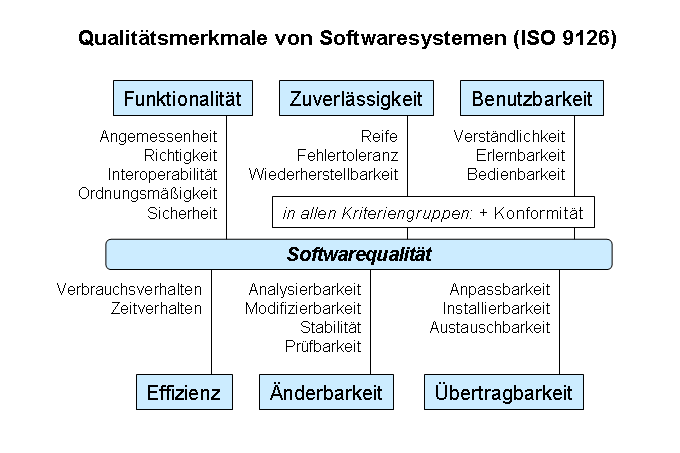
\includegraphics{Bild/ISO_9126_Grafik.png}
%	\caption{ISO 9126 Grafik Wikipedia}{ISO 9126 Grafik Wikipedia\cite{}}
%	\end{figure}
	\begin{figure}
\includegraphics{	Inhalt...}
	\end{figure}
	\subsection{Software-Ergonomie}
	„Ergonomie ist ein wissenschaftlicher Ansatz, damit wir aus diesem Leben die besten Früchte bei der geringsten Anstrengung und mit der höchsten Befriedigung für das eigene und das allgemeine Wohl ernten.“\cite[Jastrzebowski 1857]{herczeg2005software} 
	Diese älteste bekannte Definition für Ergonomie wurde 1949 durch Murell wieder aufgegriffen und unter "ergonomics" zu einer wissenschaftlichen Disziplin erhoben. Ergonomie ist ein Zusammenschluss der beiden altgriechischen Wörter ergon – Arbeit, Werk, Tat und nomos – Gesetz, Brauch, Übereinkunft. Im heutigen Sprachgebrauch wird Human Factors häufig als Synonym für Ergonomie verwendet.\cite[]{richter2010usability}
		
	„Software-Ergonomie befasst sich disziplinübergreifend mit der benutzergerechten Gestaltung der Mensch-Maschine-Interaktion sowie der Berücksichtigung der Aufgaben- und Organisationserfordernisse und der Benutzerbelange.“ \cite[S. 7]{zeidler1992software}
	Die Software-Ergonomie beschäftigt sich mit der Anpassung der Benutzerschnittstelle einer Software an die kognitiven Fähigkeiten des Menschen. Die Möglichkeiten zur Aufnahme und Verarbeitung von Informationen werden betrachtet. Die Benutzungsschnittstelle (User Interface), welche nach Herczeg\cite{herczeg2005software} die Bedienoberfläche mit den Eingabemöglichkeiten des Benutzers und den Ausgabemöglichkeiten des Computersystems darstellt, ist die Abbildung der Mensch-Computer-Kommunikation. 
	Mit Ein- und Ausgabemöglichkeiten sind die softwareseitigen Konstrukte der Dialoggestaltung wie Kommandodialoge, Menüs oder die direkte Manipulation gemeint. Dadurch findet eine wechselseitige Beeinflussung zwischen Mensch und Computer statt, die Interaktion.
	Die Software-Ergonomie hat die Motivation, den Mangel an Bedienbarkeit für die programmtechnische Benutzungsoberfläche interaktiver Computersysteme zu beseitigen. Denn versteht ein Benutzer die Art und Weise der Bedienung der Software nicht, wird er auch nicht fähig sein, ihre Vielseitigkeit zu nutzen.
	
	\subsection{Usability-Engineering}

Die Notwendigkeit von Usability Engineering lässt sich durch die beiden Aussagen "Wir alle sind Benutzer" und "Der Benutzer ist nicht wie ich" \cite{richter2010usability} sehr anschaulich begründen. Jeder von uns kommt im täglichen Leben mit verschiedenen interaktiven Produkten in Berührung, sei es im privaten Bereich mit Unterhaltungselektronik und Smartphones und den dazugehörigen Applikationen oder im beruflichen Alltag mit verschiedenen IT-Geräten und der zugehörigen Software. Die Erfahrungen fallen hier sehr unterschiedlich aus, einige Produkte lassen sich gut bedienen, andere hingegen bewerten wir als schlecht oder gar nicht benutzbar. Usability Engineering hat zur Aufgabe, die Entwicklung von schlecht benutzbaren Produkten zu vermeiden. Die zweite Aussage verdeutlicht, wie es zu eben diesen Entwicklungen kommt. Die Entwicklung von interaktiven Systemen bzw. Produkten ist ein sehr komplexer Prozess an dem Spezialisten beteiligt sind, die oftmals nicht die Sichtweise des späteren Anwenders teilen. Gerade in der Softwareentwicklung ist der Anwender für das Einsatzgebiet der Software der Experte und eben nicht der Entwickler\cite[vgl. S. 1ff]{richter2010usability}. 
		
 Zusammenfassend kann man Usability Engineering definieren als:

Usability Engineering ist die Entwicklung von Nutzungsanforderungen, Prototypen und Softwareprodukten sowie deren Validierung und Verbesserung unter systematischer Anwendung von UE-Methoden im Rahmen des benutzerzentrierten Entwicklungsprozesses.



Klarheit über den Begriff wurde durch eine allgemein anerkannte Definition in der DIN EN ISO 9241 geschaffen, welche Usability abstrakt definiert.

„Usability bezeichnet das Ausmaß, in dem ein Produkt durch bestimmte Benutzer in einem bestimmten Nutzungskontext genutzt werden kann, um bestimmte Ziele effektiv, effizient und mit Zufriedenheit zu erreichen.“ [DIN EN ISO 9241 Teil 11]

Web Usability beschäftigt sich mit dem Produkt Webseite in seinen Dimensionen Inhalt (Content-Design), Gestaltung (Page-Design) und Struktur (Site-Design		

UI Prototyping
Das UI (engl. „User Interface“, Benutzerschnittstelle) Prototyping ist eine Sammlung
von verschiedenen Methoden und orientiert sich stark am prototypischen Vorgehensmodell
(vgl. Kapitel 2.3.2). Üblicherweise werden am Anfang explorative Prototypen
eingesetzt, um das grundlegende Design der grafischen Benutzeroberfläche
(engl. „Graphical User Interface“, GUI) zu diskutieren und dem Anwender mögliche
Lösungsvorschläge vorzustellen. Ist das grundlegende Design festgelegt, wird dieses
mittels evolutionärer Prototypen schrittweise weiterentwickelt bis es den Anforderungen
des Anwenders genügt [vgl. Eller 2009, S. 78f.; DATech 2009, S. 28f.]. Die Entwicklung
von Oberflächenprototypen beginnt oft bevor eine lauffähige Version der
Software existiert, weswegen anfangs auf einfachste Mittel wie die Zeichnung mit
Stift und Papier zurückgegriffen werden kann. Mit Fortschreiten der Entwicklung kann
der Aufwand bei der Erstellung neuer Prototypen erhöht werden bis hin zum endgültigen
„Look & Feel“ der fertigen Software. Die Wahl der richtigen Darstellungsform ist
auch abhängig von der Zielstellung des Prototyps und dem damit verbundenen Arbeitsaufwand.
In der folgenden Abbildung sind drei Evolutionsstufen eines GUI Prototypen
abgebildet, angefangen von einer Stiftzeichnung über ein Drahtmodell hin
zum endgültigen Oberflächendesign [vgl. Richter et al. 2010, S. 40f.].
Abbildung 2.19:Das Usability Testing befasst sich mit Testen der Ergonomie eines Entwicklungsproduktes,
um beispielsweise den Erfolg angewendeter Usability Methoden zu bewerten.
Dabei können unterschiedliche Sachverhalte, z.B. Funktionen der Software, oder
vorher definierte Qualitätskriterien untersucht werden. Die Testmethoden sind sowohl
in der Wissenschaft als auch in der Praxis vertreten und gelten als ausgereift und
etabliert [vgl. Eller 2009, S. 71]. Beim formalen Usability Test wird zwischen einer
formativen und einer summativen Evaluation unterschieden. Die formative Untersuchung
hat die Zielstellung, die Usability Eigenschaften des zu untersuchenden Systems
zu verbessern. Die summative Evaluation dient der zusammenfassenden Qualitätskontrolle
eines fertigen Produktes. Neben den streng formalen Tests gibt es noch
zahlreiche andere Bewertungsmethoden, die weniger formal sind wie z.B. Fragebögen
oder Benutzerbefragungen [vgl. Richter et al. 2010, S. 60ff.].		
2.3.4. Gebrauchstauglichkeit
Der Begriff der Gebrauchstauglichkeit wurde bereits im vorherigen Kapitel kurz aufgegriffen
und kann als eine Definition von Usability verstanden werden. Die ISO
9241-11 beschreibt umfassend, welche Elemente und Begrifflichkeiten zum dem
Begriff der Gebrauchstauglichkeit dazu gehören und wie sie miteinander in Beziehung
stehen.
Benutzer
Aufgabe
Arbeitsmittel
Umgebung
Nutzungskontext
Produkt
Ziele
Maße der
Gebrauchstauglichkeit
Effektivität
Effizienz
Zufriedenstellung
angestrebtes Ziel
Ergebnis
der Nutzung
Gebrauchstauglichkeit
Abbildung 2.20: ISO Definition Gebrauchstauglichkeit [vgl. ISO 1998, S. 6]
2. Grundlagen und Methoden
Steffen Witte Stoffstrommodell einer Automobillackiererei Seite 41
Im Wesentlichen gehören zum Begriff der Gebrauchstauglichkeit die zu erreichenden
Ziele, der dazugehörige Nutzungskontext sowie das eigentliche Produkt, das entwickelt
oder bewertet werden soll.
Ziele
Die Ziele beschreiben den späteren Nutzen, den das Produkt dem Anwender bringen
soll. Sie können in Teilziele unterteilt werden, die sich auf bestimmte Produktkomponenten
beziehen wie z.B. spezielle Ergonomieziele für die GUI einer Software. Um
ein qualitatives Ziel wie die Gebrauchstauglichkeit eines Produktes bewerten zu können,
muss dieses operationalisiert werden. Die ISO definiert dafür Maße wie Effektivität,
Effizienz oder Zufriedenstellung. Die Effektivität setzt das zuvor definierte Ziel
des Produktes ins Verhältnis zu den Möglichkeiten, die der Anwender hat, dieses zu
erreichen. Die Effizienz setzt das Maß der Effektivität ins Verhältnis zu den benötigten
Ressourcen. Die Effizienz kann vielseitig bewertet werden, z.B. zeitlich, monetär
oder menschlich. Zufriedenstellung ist nur schwer messbar, z.B. durch subjektive
Eindrücke des Anwenders, die auf einer Skala festgehalten werden [vgl. ISO 1998,
S. 5ff.].
Nutzungskontext
Zum Nutzungskontext gehören verschiedene Elemente, wie z.B. der Benutzer, von
dem alle relevanten Eigenschaften und Fertigkeiten festgehalten werden müssen.
Handelt es sich um verschiedene Benutzertypen können Personas (siehe Kapitel
2.3.3) zur Klassifizierung eingesetzt werden. Ferner müssen die Aufgaben des Anwenders,
also die Aktivitäten mit denen die Ziele erreicht werden sollen, festgehalten
werden. Usability relevante Arbeitsmittel, die der Benutzer einsetzt, sind ebenfalls
Gegenstand des Nutzungskontexts. Dazu gehört sowohl eingesetzte Hardware als
auch zugehörige Software wie z.B. das Betriebssystem. Bei der Bewertung der
Gebrauchstauglichkeit kann die soziale, technische und physische Umgebung des
Benutzers von Bedeutung sein und muss bei Bedarf entsprechend erfasst werden
[vgl. ISO 1998, S. 5f.].
2. Grundlagen und Methoden
Steffen Witte Stoffstrommodell einer Automobillackiererei Seite 42
Gebrauchstauglichkeit ist also nicht einzig und allein die Eigenschaft eines Produktes.
Dieses ist lediglich ein Element im gesamten Bewertungsschema. Richter21 beschreibt
den Begriff der Gebrauchstauglichkeit bzw. Usability vereinfacht wie folgt
[vgl. Richter et al. 2010, S. 5]:
„Usability steht dafür, wie gut Benutzer ein Werkzeug in ihrem Umfeld zur Bewältigung
ihrer Aufgaben einsetzen können.“
Werkzeug
(Simulationsmodell)
Aufgabe
(Planung von Anlagen)
Arbeitsumfeld
Benutzer
Abbildung 2.21: vereinfachte Darstellung der Gebrauchstauglichkeit [In Anlehnung an Richter
et al. S. 4]
Am konkreten Beispiel dieser Arbeit heißt dies, dass ein Benutzer (z.B. Anlagenbetreiber
oder -planer), der nicht zwangsläufig mit der Bedienung von Stoffstrommodellen
(dem Werkzeug) vertraut ist, Simulationen im Zuge der Planungsunterstützung
durchführen kann (Aufgabe).
2.3.5. Benutzergeführte Steuerung mittels Assistent
Immer dann, wenn Spezialsoftware bei Projekten eingesetzt wird besteht die Gefahr,
dass der spätere Anwender Schwierigkeiten bei der Benutzung hat. Dies hängt vor
allem damit zusammen, dass die Sicht und Fähigkeiten des Entwicklers und die des
Benutzers sehr unterschiedlich sind. Klassische Hilfesystem oder Handbücher, die
vom Entwickler zur Verfügung gestellt werden, sind dem Anwender bei Problemen
21 Michael Richter beschäftigt sich intensiv mit der benutzerorientierten Entwicklung und ist Vorstandsmitglied
im Usability Netzwerk der Schweiz. http://www.michaelrichter.ch/, letzter Zugriff
10.11.2010
2. Grundlagen und Methoden
Steffen Witte Stoffstrommodell einer Automobillackiererei Seite 43
oder Fragestellungen behilflich. Bei besonders komplexer Software und entsprechend
komplexem Handbuch fällt es dem Anwender oftmals schwer, Antworten auf
seine Fragestellungen zu finden [vgl. Bullinger et al. 1997, S. 309]. Assistenten können
hier eine zusätzliche Hilfestellung geben.
Das Wort Assistenz stammt aus dem Lateinischen und bedeutet sinngemäß „hinzustellen“.
Entsprechend kann ein Assistent auch als „Mitarbeiter“ oder „Gehilfe“ gesehen
werden, der für den einfache Arbeitsschritte übernimmt und ihn in seiner Tätigkeit
unterstützt. Der Assistent kann den Anwender aber nicht ersetzen und übernimmt
somit nicht die Kontrolle über die Gesamttätigkeit [vgl. Steidle 2005, S. 25].
Assistenten bilden eine Weiterentwicklung klassischer Hilfesysteme, die entweder
vom Programm selbst oder vom Benutzer gestartet werden können. Sie werden direkt
während der Erledigung einer Aufgabe eingesetzt und helfen dem Anwender
durch Erläuterungen und Handlungsanweisungen eine komplexe Aufgabenstellung
zu lösen. Die Handlungsabfolge wird dabei vom Assistenten vorgegeben, um ein
strukturiertes Vorgehen zu garantieren. Diese erfolgt meist schrittweise und kann, je
nach Umfang, durch ein zusätzlich integriertes Hilfesystem ergänzt werden. Die Eingaben
des Anwenders können, soweit möglich, auf Plausibilität überprüft werden, um
Falscheingaben und daraus resultierenden falschen Analyseergebnissen vorzubeugen
[vgl. Precht et al. 2004, S. 324; Thiemann 2008, S. 12].	
		
		
		\section{Designkriterien der (Web-)Usability}
	Das Web als Werkzeug bietet dem Benutzer nicht nur eine Vielzahl von Webseiten zum Finden von Informationen, sondern immer mehr Verwaltungsaufgaben können online erledigt werden. Überzeugen kann eine solche Anwendung, wenn der Nutzer sich schnell zurechtfindet und einfach seine Ziele erreichen kann. Usability (Gebrauchstauglichkeit) ist im Web so wie bei Mobilen Anwendungen ein entscheidendes Merkmal, um sich in der Vielfalt behaupten zu können. Auch E-learning Anwendungen müssen dem Nutzer hohe Usability bieten, um als brauchbares Werkzeug bestehen zu können.\newline
				
	
		Es sind vier Faktoren zu berücksichtigen, wenn es darum geht, die Benutzungsschnittstelle benutzergerecht zu gestalten:
		
		Menschengerechte Gestaltung
		
		Im Gegensatz zu rein technischen Schnittstellen (zwischen zwei Maschinen) hat die Benutzungsschnittstelle dem Menschen Rechnung zu tragen. Der Benutzer kann mit seinen Stärken, Schwächen, Bedürfnissen und Unterschieden in der Entwicklung nur schwer formal beschrieben werden. Dennoch muss eine Anpassung der Software an den Menschen (nicht umgekehrt) erfolgen, um benutzergerecht zu sein. Dazu werden „Kenntnisse über menschliche Wahrnehmung, Denken und Problemlösen sowie über Lernen, Kommunikation und Kooperation benötigt“ [Eberleh, Oberquelle \& Oppermann 1994, S 4]. Im Abschnitt 1.3 werden einige dieser psychologischen Grundlagen vorgestellt.
		
		Aufgabenangemessene Gestaltung
		
		Software wird vom Benutzer für einen bestimmten Zweck verwendet. Meist möchte der Benutzer eine konkrete Aufgabe, insbesondere im Arbeitsleben, damit lösen. Aufgabenangemessen kann nur gestaltet werden, wenn Kenntnisse über die Aufgaben der Benutzer und ihre Vorgehensweise beim Erledigen der Aufgaben bekannt sind. Doch diese Aufgaben müssen zuerst menschengerecht formuliert werden bevor eine aufgabenangemessene Funktionalität der Software bei der Erledigung Unterstützung bieten kann. Hierzu werden Kenntnisse der Arbeitswissenschaften in der Software-Ergonomie angewandt.
		
		Technikbewusste Gestaltung
		
		Bei der Vielfalt an technischen Optionen, die heutzutage angeboten werden, fällt es nicht leicht, diese auch benutzergerecht einzusetzen. Häufig werden neue Technologien nur zum Selbstzweck eingesetzt. Für die benutzergerechte Gestaltung ist es notwendig, die verfügbaren technischen Möglichkeiten zum Wohle des Benutzers einzusetzen. Das kann bedeuten, dass der Schritt zu einer innovativen Technologie gewagt wird, oder aber etablierte, traditionelle Techniken verwendet werden. Letztlich müssen hier ökonomische und im Einzelfall auch ökologische Rahmenbedingungen bei der Entscheidung berücksichtigt werden.
		
		Organisationsgerechte Gestaltung
		
		Benutzer handeln sowohl im Arbeitsleben als auch im Privatleben meist in einem Netzwerk zusammen. Daneben findet durch die Verbreitung des Internets und der Computer auch eine technische Vernetzung statt. Diese beiden Aspekte der sozialen und technischen Vernetzung müssen durch eine organisationsgerechte Gestaltung berücksichtigt werden. Dabei muss die jeweils vorhandene organisatorische Einbindung des Softwarebenutzers beachtet werden, wenn Kenntnisse über den Menschen und seine Aufgaben gewonnen werden.
		
		Über menschengerechte und aufgabenangemessene Gestaltung existiert ein weites Spektrum fundierten Wissens durch die Forschungsarbeit der Software-Ergonomie. Die letzteren Aspekte, technikbewusste und organisationsgerechte Gestaltung, haben erst Mitte der neunziger Jahre an Bedeutung gewonnen. Als Grund dafür können die Verbreitung des Internets sowie
		
		Software-Ergonomie – theoretische Grundlagen und praktischer Einsatz Gegenstand und Ziele der Software-Ergonomie 5
		
		die Entwicklung von „haushaltstauglichen“ PCs angesehen werden. Heutzutage haben alle vier Aspekte eine große Bedeutung, wenn es um die Gestaltung neuer Software geht.
		
		Beispielsweise ermöglichen neue Technologien den Einsatz von bekannter Software in neuen Formaten. PocketPCs und die Multifunktionalität von Mobiltelefonen seien als Beispiele für Geräte genannt, die eine Anpassung der Benutzerschnittstelle an ein vergleichsweise kleines Ausgabegerät (im Gegensatz zum Desktop-Monitor) und das damit verbundene Benutzerverhalten erfordern. Technikbewusst muss auch der Einsatz von Computern als eingebettete Systeme (Embedded Systems) in modernen technischen Geräten betrachtet werden. Hinzu kommt, dass Software damit nicht mehr als grafische Oberfläche in Erscheinung tritt. Bei der Entwicklung ergonomischer Richtlinien für eingebettete Systeme verwischt die Grenze zwischen Software- und Hardware-Ergonomie zunehmend.
		
		Es sollte auch nicht vergessen werden, dass Computersysteme nicht mehr nur zur Arbeit genutzt werden, sondern auch im Freizeitbereich. Gerade hier kann die Nutzungsdauer sogar länger als am Arbeitsplatz sein, da die Software meist zum Vergnügen genutzt wird. In diesem Zusammenhang ist auch wieder die Hardware-Ergonomie gefragt, welche die körperlichen Belastungen durch lange Nutzung des Computersystems minimieren soll.
		
		Auch die veränderte Alterstruktur der Benutzer muss in der Software-Ergonomie berücksichtigt werden. Sowohl Kinder und Jugendliche als auch Senioren nutzen Computer in einem höheren Maße als noch vor einigen Jahren und stellen spezielle Anforderungen an die Hardware und Software durch ihre körperlichen und geistigen Fähigkeiten.
		
			
	
	
	
	
	\section{Benchmark Analyse E-learning und M-Learning Tools mit Usability Inhalen}
	Auf dem deutschsprachigen Markt beschränkt gibt es neben der Schulungsangeboten der vom \ac{UXQB} Anerkannten zahlreiche weitere. Es werden im folgenden nur jene aufgeführt und für den Vergleich herangezogen die ein E-learning Tool bzw. M-Learning Tool anbieten. 
	\begin{enumerate}
		\item Frauenhofer FIT (http://www.usability-ux.fit.fraunhofer.de/de/weiterbildungen-usability-und-user-experience-design/engineer-praxis.html)
		\item Usability-Academy  auch als Mobile App für Android (http://usability-academy.com/cms/unternehmen.html)
		\item http://en.tt-s.com/software/tt-knowledge-force/
	\end{enumerate}
		
	\chapter{Grundlagen E-Learning}
	\section{Lerntheorien}
	{Lernmodelle}\newline
	Für das Lernen und Lehren im 21. Jahrhundert geht das Angebot an Medien weit über reine Texte und Bücher hinaus. Entsprechend haben sich die Erkenntnisse über das menschliche Lernverhalten entwickelt. Der rein behavioristische Ansatz \cite[John Watson/ B.F.Skinner]{baumgart1998entwicklungs} wurde von den kognitionspsychologischen Lernmodellen \cite[S.102]{arnold2013handbuch}abgelöst. Beim ersten Modell wird Lernen als Veränderung von Verhaltensweisen durch Verstärkung von erwünschtem Verhalten verstanden. Durch Versuch und Irrtum oder durch Beobachtung eines Vorbildes(sog. Modellpersonen) und regelmäßiges Wiederholen können neue und komplexe Verhaltensweisen angeeignet werden\cite[S.101 Skinner]{arnold2013handbuch}. Wissen sind externe Fakten und der Prozess des Denkens- und Verstehens wird als "Blackbox" hingenommen. 
	Durch 4 Arten von Verstärken kann auf den Erfolg Einfluss genommen werden: 
	\begin{itemize}
		\item materielle Verstärker z.B. Geld, Eis
		\item soziale Verstärker z.B. Lob, Anerkennung
		\item Aktivitätsverstärker z.B. etwas machen dürfen wie Pause oder Urlaub
		\item informativer Verstärker z.B. Rückmeldung über die Richtigkeit einer Antwort, über die Lerngeschwindigkeit
	\end{itemize}\cite[S.21]{issing2009online}
	Ein typischer Programmablauf eines auf dem behavioristischen Modell basierenden System sind Frage-Antwort-Sequenzen mit sofortiger Rückmeldung. Der Schwierigkeitsgrad steigt Linear und es können keine Teile des Programms übersprungen werden. Diese Variante von Lernprogrammen werden als Drill-and-Practice-Programme bezeichnet. Hauptkritik an den meist aus Tierexperimenten und Laborversuchen gewonnenen Erkenntnisse ist, dass diese nicht zwingend auf aktuelle E-Learning Umgebungen übertragbar sind.
	Auch wenn die behavioristische Lerntheorie nicht das aktuellste Modell darstellt, finden die aufgeführten Verstärker, strikt lineare Abfolgen und ständige Wiederholungen im Bereich der webbasierten Lernangebote Anwendung zum Beispiel bei Vokabellernprogrammen. Ein großer Vorteil dieser Programme ist, dass Sie meist nach eigenem Tempo durchlaufen werden können\cite[65 ff.]{niegemann2005}. 
	
	Die kognitionspsychologischen Ansätze gehen auf den Menschen und seine Fähigkeit Informationen aufzunehmen und zu verarbeiten ein. Der Prozess des Lernens von der Wahrnehmung über die Bildung kognitiver Schemata und mentaler Modelle sind die Grundpfeiler kognitiver Lernmodelle. Lernen ist somit ein Informationsverarbeitungsprozess. Diesem Lernmodell liegen einige Annahmen zugrunde: 
	\begin{enumerate}
	\item Der Mensch als Informationsverarbeitungssystem hat zwei Kanäle, die visuelle/bildhafte und die auditive/verbale Informationsaufnahme. 
	\item Die zweite Annahme ist, dass das Gedächtnis eine begrenzte Kapazität für die Verarbeitung von Informationen hat.   
	\end{enumerate} 
	Ziel bei der Gestaltung von Lernmaterialien ist es, nach Möglichkeit beide Kanäle bei der Verarbeitung von Informationen zu aktivieren den Lernenden jedoch nicht mit zu vielen Informationseinheiten kognitiv zu überreizen. \cite{baumgart1998entwicklungs}
	Bezogen auf multimediales Lernen, ist die Erkenntnis, die hervorgehoben werden soll, dass die bildhafte Darbietung von Informationen mentale Modelle fördert und somit das Lernen erleichtert.
	
	Um zu einem mentalen Modell zu gelangen, bedarf es des Aufbaus diverser Strategien, Wissen zu strukturieren. Diese haben verschiedene Strukturen zum Inhalt:
	
	Verarbeitungsstrukturen: Diese Strukturen können beispielsweise Kausalketten mit entsprechenden Erläuterungen der einzelnen Ursache-Wirkungs-Elemente umfassen.
	Vergleichsstrukturen: Sie lassen sich als Matrizen darstellen, die den Vergleich zweier oder mehrerer Elemente anhand mehrerer Dimensionen ermöglichen.
	Generalisierungsstrukturen: Diese repräsentieren als eine Art Baumstruktur den Kerngedanken mit seinen untergeordneten ergänzenden Details.
	Aufzählungsstrukturen: Sie betreffen eine Liste, die aus einer Zusammenstellung von Einzelelementen besteht.
	Klassifikationsstrukturen: Diese Strukturen sind hierarchisch angeordnet und umfassen Gruppen und Untergruppen.
	
	Aktuell dominiert das konstruktivistisch Problem basierte Lernmodell, welches das kooperative lernen als Verstärker nutzt. Bei ersterem geht es um den Aufbau von Wissen durch Verknüpfung von neuen Informationen mit bereits vorhandenem Basiswissen.\cite[S.30-32]{issing2009online}. Diesem Ansatz nach, muss immer auf den Einzelnen eingegangen werden, da das Vorwissen von Person zu Person variiert. 
	Webbasierte, interaktive E-learning Angebote %wie das Glossar zur Basiszertifizierung CPUX-F des UXQBU 
	werden diesem Lernmodel sehr gut gerecht: Die Lernenden können dort einsteigen, wo Sie wollen und der Zugang ist wahlweise über Smartphone, Tablet oder PC möglich. 
	
	Lernen im Konstruktivismus wird verstanden als die Konstruktion von Wissen auf der Basis individuellen Vorwissens; -> daher muss immer auf den einzelnen Lernenden Eingegangen werden. \cite[S.30ff]{issing2009online}
	
	Der Begriff Konstruktivismus wird im E-Learning Kontext von verschiedenen Forschern unterschiedlich definiert. Im Folgenden soll darunter ein Lernansatz verstanden werden, der Lernende als selbstverantwortliche, aktive Personen im Hinblick auf ihren Wissenserwerbsprozess begreift (Loyens und Gijbels, 2008). Konstruktivistische Lernumgebungen beinhalten mehrere Merkmale, die den Lernprozess unterstützen sollen (Loyens und Gijbels, 2008):
	
	Merkmale konstruktivistischer Lernumgebungen
	
	Wissenskonstruktion: Konstruktivistische Lerntheorien betonen die aktive Konstruktion von Wissen. Konkret bedeutet dies: Lernende interpretieren und transformieren neue Informationen auf Basis bereits erworbenen Wissens, welches von den Lernenden aktiv abgerufen wird.
	Kooperatives Lernen: Eine weitere wichtige Grundannahme bezieht sich auf das gemeinschaftliche (kollaborative) Lernen mit anderen Lernern, Lehrern und weiteren Personen, durch welches die Wissenskonstruktion unterstützt werden soll (vgl. Schaumburg und Issing, 2004). Besonders beim Lernen mit anderen Lernenden nimmt man die Lernförderlichkeit aufgrund ähnlicher Verständnisniveaus an.
	Selbstregulation: Unter Selbstregulation werden eine Reihe von Teilaspekten subsumiert. Beispielsweise fallen hierunter die metakognitiven Fähigkeiten, wie das Setzen von (Lern-)Zielen, aber auch Selbstbeobachtung, Selbstbewertung und Selbstverstärkung während des Wissenserwerbs (vgl. auch Narciss, Proske und Koerndle, 2007).
	Authentische Lernsituation: Im Kontext konstruktivistischer Lerntheorien sollten Lernsituationen vorzugsweise praxisbezogen bzw. authentisch sein. Hierzu können Lernende mit komplexen, schlecht strukturierten Problemen konfrontiert werden – ähnlich den Problemsituationen, die sie auf ihrer zukünftigen Arbeitsstelle antreffen. Vielschichtige Probleme zeichnen sich durch zahlreiche interagierende Elemente und der Möglichkeit multipler Lösungsansätze aus. Im Zusammenhang solcher Problemsituationen wird auch häufig vom entdeckenden Lernen (discovery learning) gesprochen.
	Konstruktivistische Lerntheorien werden vor allem in der populärwissenschaftlichen Literatur vehement vertreten (vgl. z.B. Kirschner, P. A., Sweller und Clark, 2006), wenngleich dort in aller Regel nur sehr vage Definitionen existieren. Auch in wissenschaftlichen Fachartikeln ist eine klare Begriffsbestimmung nur selten aufzufinden (Loyens und Gijbels, 2008).
	%Gefördert werden soll ein problemlösendes Denken,
	
	Konnektionismus
	Definition: Konnektionismus
	
	Konnektionistische Modelle bestehen aus vielen einfachen Einheiten, die miteinander vernetzt sind. Eine häufig verwendete Realisierung konnektionistischer Modelle sind künstliche neuronale Netze. Häufig werden die Begriffe Konnektionismus und (künstliche) neuronale Netze auch gleichgesetzt. Neuronale Netze stellen einen Oberbegriff dar, der zahlreiche, zum Teil sehr unterschiedliche Modelle umfasst (Rey und Wender, 2008; siehe auch www.neuronalesnetz.de). Diese Modelle können unter anderem dazu eingesetzt werden, menschliches Verhalten und Erleben bzw. die diesen zugrunde liegenden Gehirnprozesse (am Computer) zu simulieren und dadurch besser zu verstehen. Sie lassen sich aber ebenso als statistische Verfahren bei der Datenauswertung einsetzen. Aufgrund der Fülle der Anwendungsbereiche ist verständlich, warum keine allgemein anerkannte Definition zu neuronalen Netzen existiert. Gemeinsam ist den verschiedenen Modellen aber, dass bei diesen – wie bei anderen statistischen Verfahren auch – Matrizenberechnungen durchgeführt werden und dabei Informationen aufgenommen, verarbeitet und ausgegeben werden (Rey und Wender, 2008):
	
	Schematische Darstellung eines neuronalen Netzes
	Abbildung 7: Schematische Darstellung eines neuronalen Netzes
	Informationsaufnahme: Zunächst werden dem Netz (wiederholt) Informationen in Form von Zahlen als Eingabe zur Verfügung gestellt.
	Informationsverarbeitung und Netzmodifikation: Mit Hilfe dieser "Zahlenbündel" und bestimmter Umformungsregeln wird das Netz verändert. Die Veränderung des Netzes, d.h. der Lernprozess, findet typischerweise in einer Vielzahl von Schritten statt. Die dazu notwendigen – oftmals sehr umfangreichen – (Matrizen-)Berechnungen werden an Computern vorgenommen. Während und nach den Berechnungen zur Umformung des Netzes durchlaufen Informationen das neuronale Netz. Diese Zahlen werden durch das Netz modifiziert und verlassen dieses anschließend wieder – ebenfalls in Form eines Zahlenbündels.
	Informationsausgabe: Die Informationsausgabe stellt die "Antwort" des Netzes auf die vorangegangene Eingabe dar.
	Gemeinsamkeiten und Unterschiede zum Kognitivismus
	
	Neuronale Netze besitzen somit Gemeinsamkeiten zu kognitiven Modellen, da auch dort Informationen aufgenommen, verarbeitet und wieder ausgegeben werden. Während kognitive Modelle traditionell eher die Gemeinsamkeiten mit dem Computer hervorheben, betonen neuronale Netze vornehmlich die Unterschiede zwischen Menschen und (heutigen) Computern bei der Informationsverarbeitung und wurden zudem durch das menschliche Gehirn als "Vorbild" inspiriert (Rey und Wender, 2008). Konnektionistische Modelle kamen im Gegensatz zu kognitiven Modellen in der E-Learning Forschung meines Wissens nach bisher nicht zum Einsatz, obwohl sich der Rückgriff auf diese Ansätze unmittelbar anbieten würde.
	
	Kritik und Würdigung
	
	Die Simulation menschlichen Lernens mittels neuronaler Netze wird unter anderem hinsichtlich ihrer fragwürdigen biologischen Plausibilität kritisiert. Viele neuronale Netze widersprechen biologischen Grundannahmen und sind daher als Modelle zur Erklärung menschlichen Lernens nur bedingt geeignet (Rey und Wender, 2008). Allerdings trifft dieser Kritikpunkt meist in noch stärkerem Maße auf behavioristische, kognitive und konstruktivistische Modelle zu. Neben der fragwürdigen biologischen Plausibilität besitzen einige neuronale Netze aufgrund ihrer zahlreich enthaltenen Parameter und Variablen die Gefahr, jede denkbare menschliche Verhaltensweise beim Lernen abbilden zu können. Dadurch wäre das Modell nicht mehr falsifizierbar, d.h. nicht mehr durch empirisch gewonnene Daten widerlegbar, sondern könnte durch die Wahl geeigneter Parameter immer vor der Falsifikation geschützt werden (vgl. Popper, 1996; Rey und Wender, 2008). Trotz dieser und weiterer Kritikpunkte wurden neuronale Netze bereits in vielen Bereichen inner- und außerhalb der Psychologie erfolgreich eingesetzt (Rey und Wender, 2008). Der Einsatz neuronaler Netze als Erklärungsansatz zum menschlichen Lehren und Lernen mittels elektronischer Medien erscheint schon deshalb äußerst ergiebig, weil Begriffe wie Lernen und Wissenserwerb bei beiden eine zentrale Bedeutung einnehmen. Insofern plädiere ich für eine Verknüpfung dieser beiden Forschungsgebiete.
	
	\section{E-learning}
	\subsection{Begriffsdefinition E-Learning}
	Auf der deutschen Wikipedia Seite wird die Definition von Michael Kerres aufgegriffen:
	"Unter E-Learning (englisch electronic learning = „elektronisch unterstütztes Lernen“, wörtlich: „elektronisches Lernen“), auch als E-Lernen (E-Didaktik) bezeichnet, werden alle Formen von Lernen verstanden, bei denen elektronische oder digitale Medien für die Präsentation und Distribution von Lernmaterialien und/oder zur Unterstützung zwischenmenschlicher Kommunikation zum Einsatz kommen.
	Für E-Learning finden sich als Synonyme auch Begriffe wie: Online-Lernen (Onlinelernen), Webbasiertes-Lernen, multimediales Lernen, computergestütztes Lernen, Computer Based Training, Open and Distance-Learning u. a."\cite{kerres2005learning}
	
	Auf der amerikanischen Webseite elearners.com  ist E-Learning mit dem Kriterium der Netzbasiertheit definiert:
	„Any learning that utilizes a network (LAN, WAN or Internet) for delivery, interaction,
	or facilitation. This would include distributed learning, distance learning (other
	than pure correspondence), CBT delivered over a network, and WBT. Can be synchronous,
	asynchronous, instructor-led or computer-based or a combination.“\cite{aldrich2003simulations}
	
	Die Bedeutung des Begriffs elektronisches Lernen hat sich vom Lernen mit Fernsehen, Videoband und CD-ROM am Computer zum Netz gebundenem bzw. webbasiertem Lernen entwickelt. 
	Daraus wird deutlich, dass der Gebrauch des Begriffes von der Zeit abhängig ist. Der aktuelle Gebrauch ist als Überbegriff für alle Arten medienunterstützten Lernens.\cite[S.22 ff.]{baumgartner2002learning} Im Rahmen dieser Arbeit wird E-Learning mit dem Lernen über Internet bzw. webbasierte Anwendung verstanden. 
	
	
	Eine Vorlesung ohne Power Point und PDF-Handouts ist undenkbar geworden. Mit dem Angebot an neuen Medien hat sich auch eine neue interaktivere Lernkultur entwickelt, die neue Anforderungen an die didaktische Aufbereitung der Lehrinhalte stellt. 
	
	\subsection{Gestaltungsprinzipien für E-learning Angebote}
	Zielgruppe ist intrinsisch motiviert. Bzw. Die Motivation ist nicht relevant für die Gestaltung des E-learning. Lediglich die Erhaltung bzw. Steigerung der anfangsmitivation
	Synergien durch arbeiten am Arbeitsplatz und im Kreise von Kollegen
	
	\textbf{Design Prinzipien}
	
	Prinzipien des systematischen Instruktionsdesigns = Gestaltungsorientiertes Mediendidaktik
	folgen der kognitive und kostruktivistischen Auffassung des Lernens. 
	
	\subsection{Ausgewählte Methoden des E-learning}
	
	
	
	\subsection{\ac{LCMS} und \ac{LMS}}
	
	\textbf{Autorensoftware} auch: Autorentool, Autoren- oder Authoring-System; engl.: authoring software) soll die Erstellung multimedialer Anwendungen insbesondere im E-Learning-Bereich für die Autoren dieser Anwendungen erleichtern.
	Mit der Software werden die Autoren in ihrer Arbeit unterstützt. Von den Autoren werden keine umfassenden Programmierkenntnisse verlangt, um Trainingskurse für Web Based Training, Computer Based Training oder entsprechende E-Learning-Module zu erstellen.
	Die Autorensoftware erleichtert die Erstellung interaktiver Präsentationen und Animationen, auch von komplexen Multimedia-Anwendungen. Interaktionen (z. B. Reaktionen auf Benutzereingaben oder Mausklicks) und Animationen (z. B. Bewegung von Elementen) können im Idealfall intuitiv erstellt werden. Die Integration von multimedialen Elementen ist ebenfalls möglich.
	Beispiele für Autorensoftware sind Adobe Authorware, Lectora, IMC Content Studio, IDA oder das Opensource-Produkt eXe-Learning. %Wiki
	
	%What are the differences between LMS, LCMS, and CMS? This question often elicits confusion among those shopping for the right software tools for their organization. Not to worry—we know the difference and we are going to share our knowledge.
	%First, let’s define our abbreviations. “LMS” is an acronym for “Learning Management System”, a software platform used to deliver and track training courses. “LCMS” stands for “Learning Content Management System”, or software used to author and manage learning content. Finally, a “CMS” is a “Content Management System”, or software used to organize content comprising a website.
	%Whether you are an elearning novice or an experienced training director, you should understand these systems to know which tools you need in your learning and development program. Let’s clarify the differences:
	%What is a Learning Management System?
	%Commonly used in corporate training and higher education settings, learning management systems are software platforms that store and deliver training content and then track participation in training. Most LMS enable learning managers to upload online training content created by a variety of authoring tools, as long as the content is compliant with SCORM, the industry standard file format. An LMS then allows companies to assign training to their employees, track their participation, and produce documentation of employee training activity and results. In sectors where companies are legally required to provide certain types of safety or compliance training, an LMS is an essential tool to keep track of the company’s compliance.
	%Finally, using an LMS enables companies to create different tracks of training courses to deliver to different groups of employees in order to fulfill their specific training objectives—creating a customized learning program for each employee, as needed. In addition to delivering and tracking online training courses, many LMS enable training managers to keep track of employees’ participation in other types of training programs, such as in-person classes.
	%Bluevolt, Litmos, and Topyx are examples of a few learning management systems.
	%What is a Learning Content Management System?
	%In contrast to an LMS, learning content management systems are primarily used to create, store and organize elearning content. Instructional designers use this software to develop, manage and publish training content. Rather than creating course catalogs for wide audiences, LCMS platforms allow single courses to be modified for individual learners.
	%An LCMS system usually allows multiple collaborators to work together to create content that can then be published in a variety of formats. The key difference between an LMS and an LCMS is the target user. The LMS user is the learner, while the LCMS user is the learning content creator.
	%
	%Many LCMS also have the ability to store and deliver older versions of courses. Companies that want customized courses delivered to their employees generally use an LCMS. When designing training materials to deliver through an LCMS, learning and development personnel should research quality authors and publishers. Xyleme and Kenexa are two examples of learning content management systems.  
	%
	%What is a Content Management System?
	%
	%Content management systems create the framework in which content is stored and displayed on a website. These systems manage various content forms, including files, images, electronic documents, audio files, and many more.
	%
	%CMS functions allow distributors to decide which content is displayed privately or publicly. Content can be easily tagged using metadata, which is best for searching and using content quickly and efficiently. Drupal and WordPress are popular content management systems used to create all kinds of websites. As opposed to a CMS, a learning CMS is specialized for the creation and management of learning content.
	%
	%Management Systems in Summary
	%
	%You have the ability to manage and deliver content on all three management systems. While these management systems have several similarities, they ultimately have different functions.
	%
	%Take some time to study these similarities and differences to avoid using the wrong acronym in professional discussions. As soon as you start using these acronyms in discussions...you're going to sound like an elearning pro.
	%
	%Which management system do you use for your team? Share with us in the comments.\cite{LMS_LCMS}
	\section{M-Learning}
	
	\section{Gamification als Instrument des E-Learning}
Game play helps to exercise (and motivate) our mental muscles.
Believe it or not, playing games is actually good for your brain. Not only does it help to engage learners in the eLearning process itself, but it also serves to remedy the boredom that so often leads to unsuccessful learning experiences (Free eBook - How Gamification Reshapes Learning). A report that was released by Leicha Bragg of Deakin University details a study that was conducted in three different schools, which involved 240 students [5].According to the research, students were more motivated to learn mathematics when the information was presented in a gaming format. Even their attitude toward the subject changed, as did their confidence regarding the various concepts involved. The students were also more motivated to learn the information, which improved their overall success and alleviated the boredom that is often associated with repetition (especially relating to problem solving).\cite{BrainFact}	
	

	
	\chapter{Konzeption} //Skizzierung dessen was kommt 
%\centering{75\% aller Software-Mängel werden während der Entwicklung verursacht.\\
%Davon bleiben 80\% bis zur Nutzung unerkannt.}\cite[Software Quality Systems, Köln]{rudlof2006handbuch}

	\section{Rahmenbedingungen}
	Innerhalb des KOMET Projektes soll ein E-Learning Tool entwickelt werden, welches das selbst gesteuerte Lernen erleichtert und als begleitendes Material/Medium dient. 
	Die Grundidee, ist die Gestaltung eines Quiz mit der Option sich sozial zu vernetzten nach dem Modell von Quizduell. 
	
	 bei dem die Zeit und die Folge von richtigen Antworten aufgezeichnet werden und in den Highscore einfließen.
	E-learning tool was Entwicklern das beachten von Usebility bei der Entwicklung von BUIS erleichtern soll.  
	
	%Auch unternehmen suchen nach Möglichkeiten Ihre Mitarbeiter zu schulen und die dank spielerisch gestalteten E-learning tools. 
	%Usability Wissen soll so interessant aufbereitet werden, dass es spielerisch aufgenommen werden kann. Das Lernen und verinnerlichen von Usability bei der Entwicklung von Software soll innerbetrieblich gepflegt werden können. 
	%Der Content sollte leicht und intuitiv aufbereitet sein. Für die vielseitige Verwendbarkeit. Spielerisch und Sozial vermitteln was relevant ist für die Entwicklung von Benutzerfreundlichen Anwendungen und Seiten.
	
	%%
	%% Hochschule für Technik und Wirtschaft Berlin, Deutschland; 2artop - Institut an der Humboldt-Universität zu Berlin, Deutschland
	% Mit dem Glossar zur Basiszertifizierung CPUX-F des UXQB steht eine Sammlung von Definitionen zu grundlegenden Begriffen und Konzepten aus dem Fachgebiet Usability und User Experience zur  Verfügung. Zur Erleichterung der Auseinandersetzung mit dieser Begriffswelt wurde ein webbasiertes Hypertextsystem erzeugt, das wahlweise über Smartphone, Tablet oder PC benutzt werden kann. Um den Lernanreiz zu erhöhen wurde zusätzlich ein Frage-und-Antwort-Spiel mit einer Highscore-Liste entwickelt. Dieses so genannte „Usability-Quiz“ wird im Rahmen des Vortrags erstmals öffentlich vorgestellt. Geplant ist anschließend eine „Birds of a Feather“-Session, um die Herausforderungen der Weiterentwicklung zu einer sozialen Anwendung analog zur mobilen App „Quizduell“ zu diskutieren.
	%
	3 Ideen, 
	1. Glossar, konkrete Beschreibung zum lernen langweilig, Kategorisierung der Begriffe und Definitionen, 
	2. Quiz, gegen Maschine bzw. einfache Lern, zum lernen für die Zertifizierung,
	3. Quizduell, gegen andere direktes Duell, 
	
	Glossar beinhaltet Worte der Zertifizierung Seminar: Zielgruppe? 
	Glossar zum lernen in Bereiche aufgeteilt, Usability Quiz zum testen seiner bereits gelernten Erfolge, 
	Branding soll noch gemacht werden mit dem Augenmerk der Informationsgestaltung Aufbereitung
	\begin{itemize}
		\item{Webbasiertes Tool}
		\item{HLMT/ HTML 5}
		\item{Jason/ Java Skript/ Python}
		\item{Vokabeln plus Definitionen}
		\item und einige mehr  
	\end{itemize}
	
	Anforderungen an die Software = Lernerfolge testen, Schwierigkeitsgrad, 
	
	\subsection{Glossar sequentiell}
	\subsection{Glossar shuffle}
	\subsection{Begriff + Definition + Bild}
	\subsection{Quiz gegen einen Gegner direkt?}
	\subsection{Fragen}
	Welches Spiel/Welche Methode
	\begin{enumerate}
		\item  ist am einprägsamsten?
		\item  ist für zwischendurch?
		\item  hat Ihnen am meisten Spaß gemacht?
		\item  ist am Zeitaufwendigsten?
		\item  ist der Fortschritt/Lernerfolg am besten erfasst?
		\item Inhalt...
	\end{enumerate}
	
	\section{Zielgruppe}
	Die Zielgruppe des Usability - Quiz sind Menschen mit einer Vorqualifizierung. Sie sind routiniert am Computer und zählen diesen zu Ihrem täglichen Arbeitswerkzeug. 
	Ihr Auge ist geschult im surfen durch das Web und Selektieren von relevanten Informationen. 
	Entwickler und andere Personen die sich seriös für Usability und User Experience interessieren und hierfür weiterbilden möchten. 
Zielgruppe interessierte mit heterogenen Vorwissen	
	Zielgruppen
	Die Zielgruppe sind Usability Professionals und die, die es noch werden möchten. 
	\section{Seminarplanung}
Lerninhalte sollten nicht Änderungsanfällig sein, bzw. Jede Überarbeitung der Inhalte erfolgt per Hand. Nur auf festgesetzte Inhalte nutzbar, da kein Backend vorhanden für die Überarbeitung

	\subsection{Inhalt und Ziel des Seminars}
	Vermittlung des
	\subsection{Funktionale Anforderungen}
	Darbietung der Begriffe, Verlinkung zu Synonymen, 
	Dazu wurde das Glossar zu einer Art Wiki aufbereitet und zum Prüfen des bereits erworbenen Wissens ein Lern-Quiz in der Art einer Vokabeltrainings entwickelt. Zu der gegebenen Definition gilt es zwischen 4 Antwortmöglichkeiten den richtigen Begriff zu wählen. Die besten Ergebnisse finden zugang in die Top 10 der Highscore Liste die mit implementiert wurde um einen weiterer Anreiz für das so genannte Usability-Quiz zu schaffen. 
	Evaluieren des Quiz nach Usability Richtlinien?
	
	Open Source
	CourseBuilder (Webbasiert) 
	
	\subsection{Quiz}
	\subsection{Lückentext}
	\subsection{Memory}
	
	%\begin{itemize}
	%	
	%	\item Wie können Inhalte (Usability Glossar) vermittelt werden?
	%	\item Was soll vermittelt werden? Aufbereitung des Content als Lückentext, Bildaufgabe, T
	%	\item Wer sind die Zielpersonen Benutzer?
	%	\item BUIS sind nicht intuitiv und selten eingebungen, folgen, werden ungern genutzt
	%	\item Ein E-learning Tool welches spielerisch in Leerlaufphasen genutzt werden kann
	%	\item E-learning Plattform als Autorenprogramm um Inhalte auf BUIS anpassen zu können
	%	\item Es gibt kein Know How bei den KMU entwicklern
	%	\item keine Ansprechend aufbereiteten Inhalte um sich Usability anzueignen
	%	\item Was gibt es auf dem Markt und warum ist das Thema noch nicht angenommen
	%	\item Angebote die verfügbar sind noch nicht angenommen und wie müsste das Spiel aufgebaut sein damit sich KMU Entwickler damit beschäftigen
	%	\item Innerhalb des KOMET Projektes gibt es bereits folgenden Prototypen und 
	%\end{itemize}
	
	
	\section{\ac{LCMS} Wahl}
	Framework als Entwicklungsumgebung oder doch nur Mokups? 
	Autorenprogramm
	
	Powertrainer / Lecturnity 
	Adobe Captivate (bzw. die gesamte eLearning Suite 2) 
	Lectora Publisher 
	Outstart Trainer 
	SumTotal Toolbook 
	digital spirit elearning studio  
	
	
	
	\section{Auswertung}
	\section{Zusammenfassung} 
	Autorenprogramm = Quatsch, nur für den Prototypen zur Visualisierung der angestrebten funktionalitäten
	
	Aussicht für die Umgebung auch als Autorentool anwendbar? Wie ist die Software zu strukturieren um den Content erweiterbar bzw. einfach veränderbar zu machen. 
	
	
	\chapter{Praxisteil}
	\section{Erweiterung des KOMET Code durch Kategorisierung}
	\section{Erweiterung des KOMET Code durch Bilder für 98 Begriffe}
	\section{Prototyp Kombinations/ Zuordnungspiel}
	
	%\addchap{Quellen}
	\printbibliography
%	[heading=subbibliography,title=Literatur,nottype=Web]
%	\printbibliography[heading=subbibliography,title=Internet,type=web]
%	
\end{document}